\chapter{基于语义识别的自动配色方案辅助设计工具}

\section{系统结构}

本系统的算法实现结构如图~\ref{figure:内部实现逻辑}

\begin{figure}[!htbp]
\centering
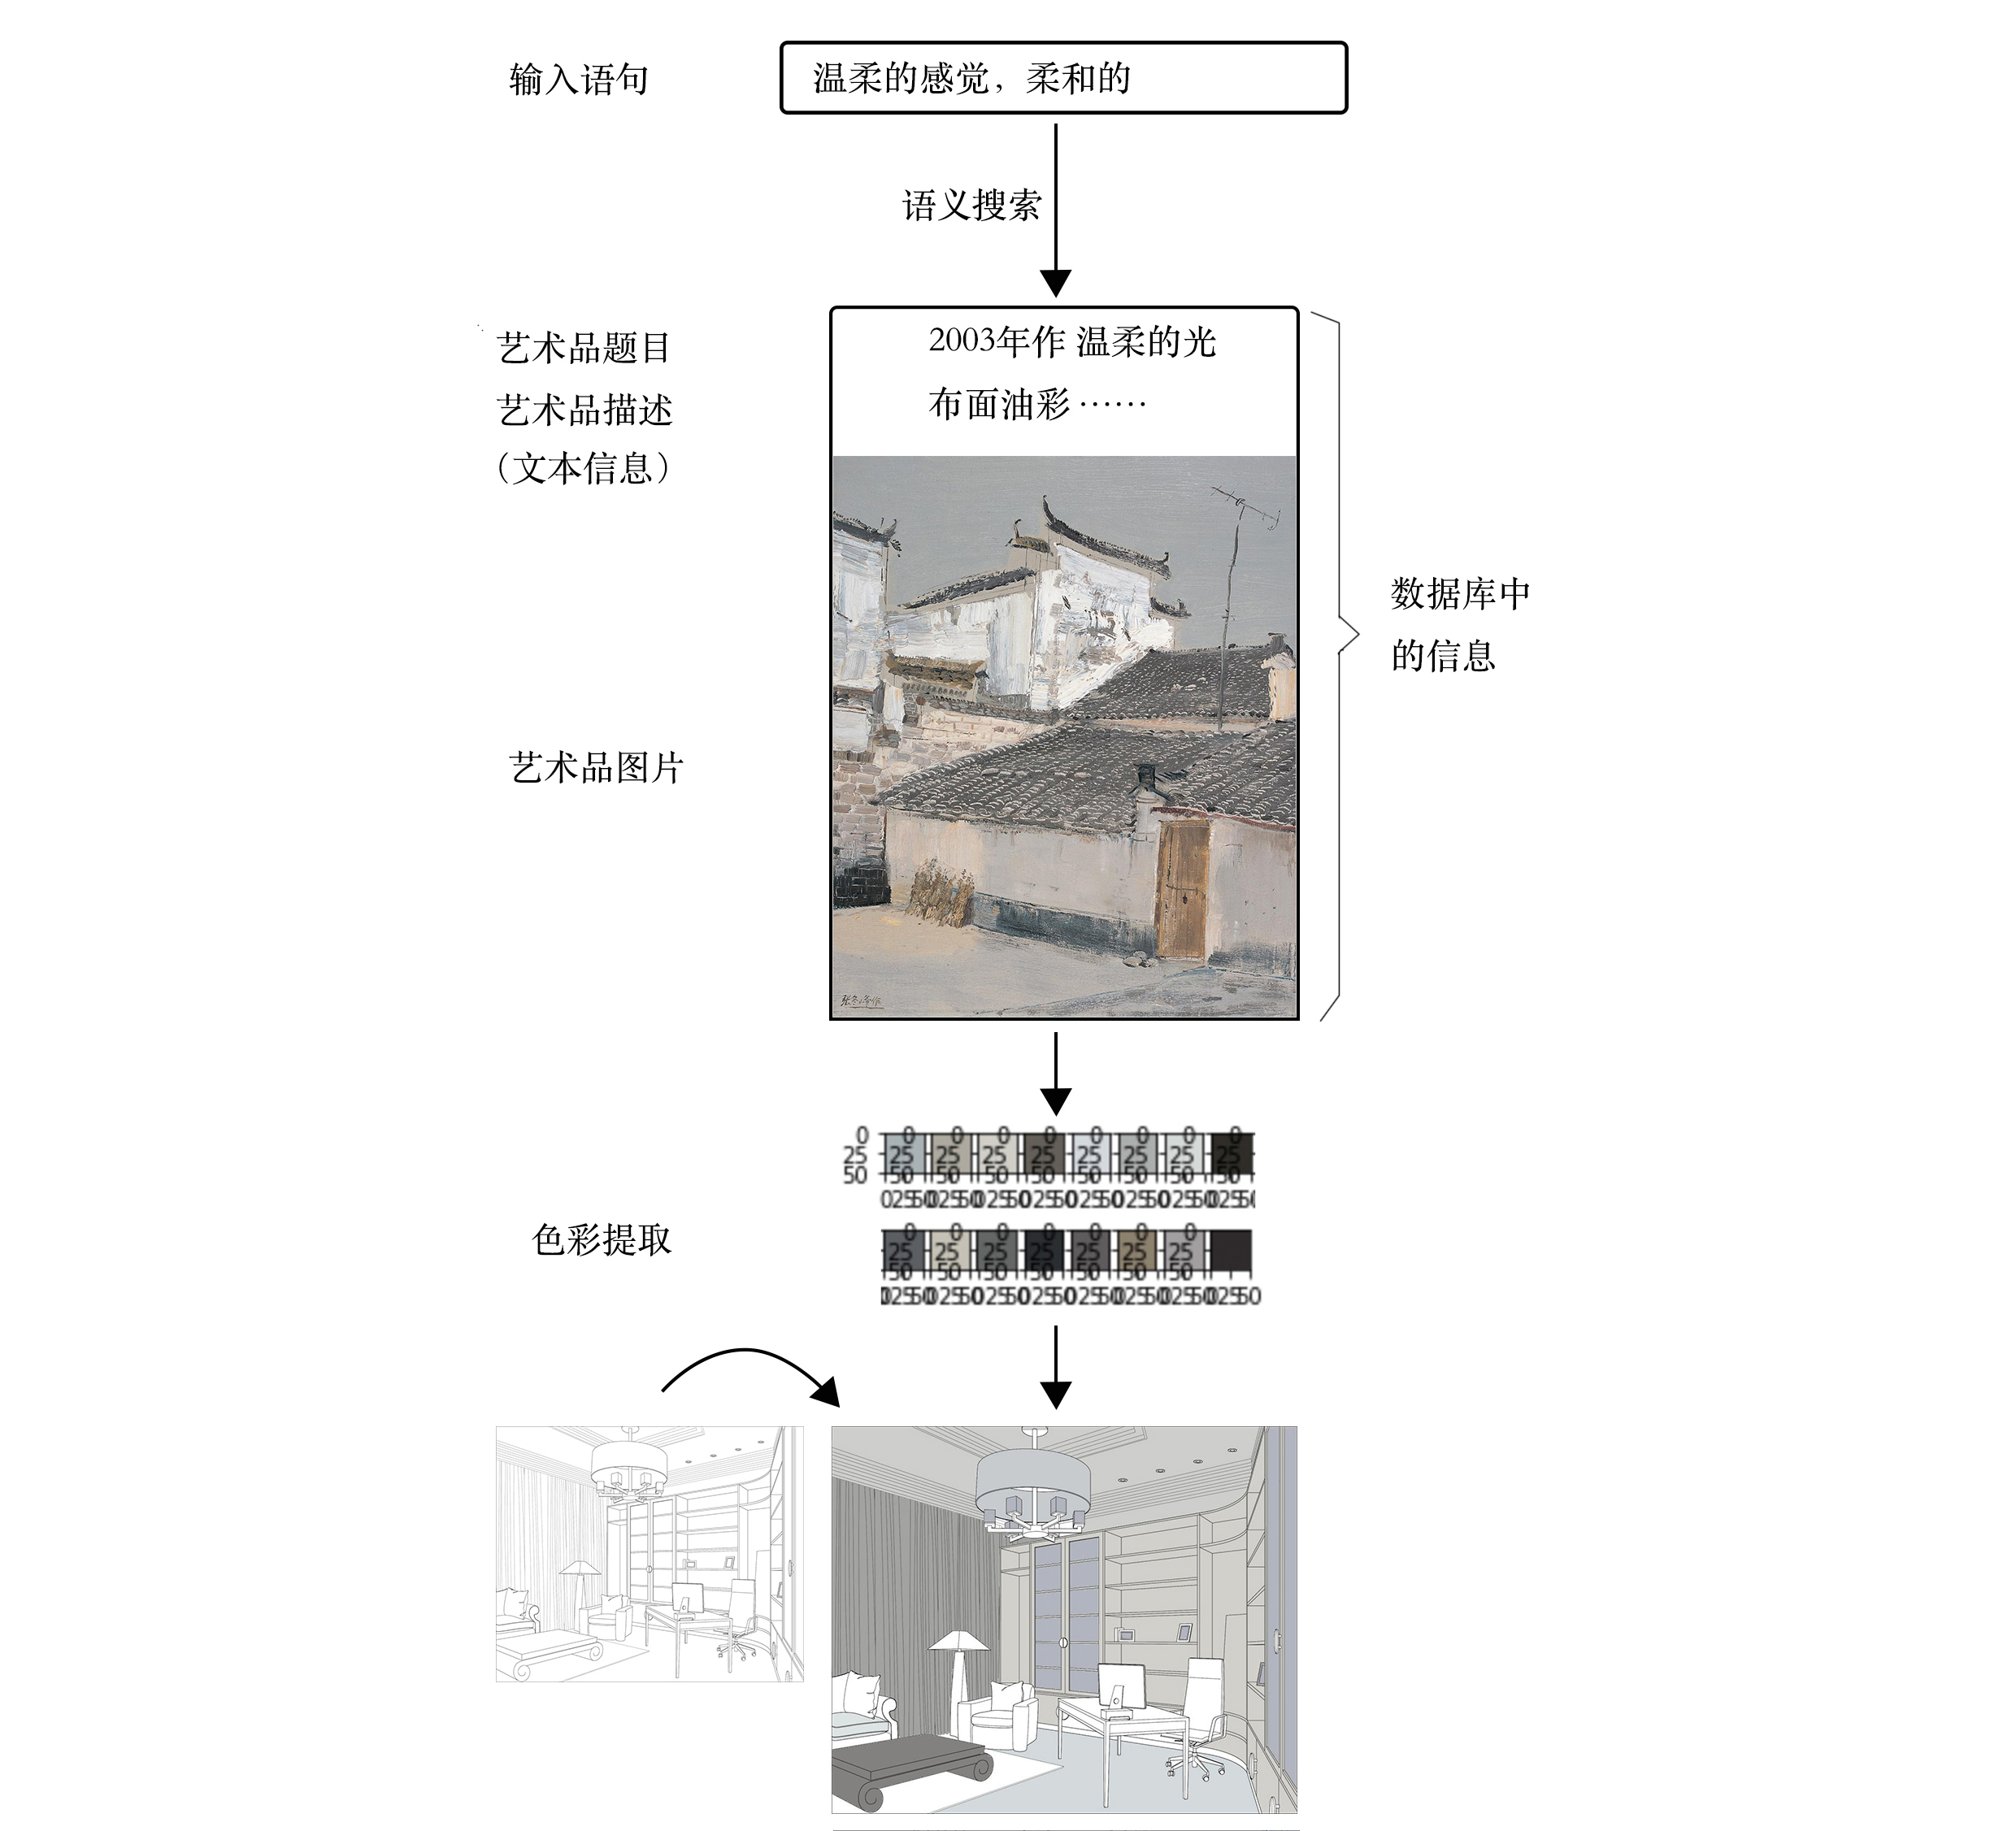
\includegraphics[width=\linewidth,keepaspectratio]{data/chapter-1/系统内部逻辑.jpg}
\caption{内部实现逻辑}
\label{figure:内部实现逻辑}
\end{figure}

本系统的整体思路为:首先,输入语句是对需求的文本描述,可以是词语,句子或不完整的句子。第二步,针对输入语句对艺术品的文本信息进行语义搜索,找出与之关联度高的艺术品文本信息。第三步,依据艺术品数据库中艺术品的图片信息和文本信息的隐藏信息关联匹配对应,即可以找出与输入文本关联度高的图片。之后,从图片中提取色彩方案,包括绘画作品的色彩和配色比例。最后,将提取的色彩方案运用到设计效果图上预览。

本系统的用户交互框架如图~\ref{figure:用户逻辑},对于用户来说,用户的使用逻辑是简单而清晰的,

\begin{figure}[!htbp]
\centering
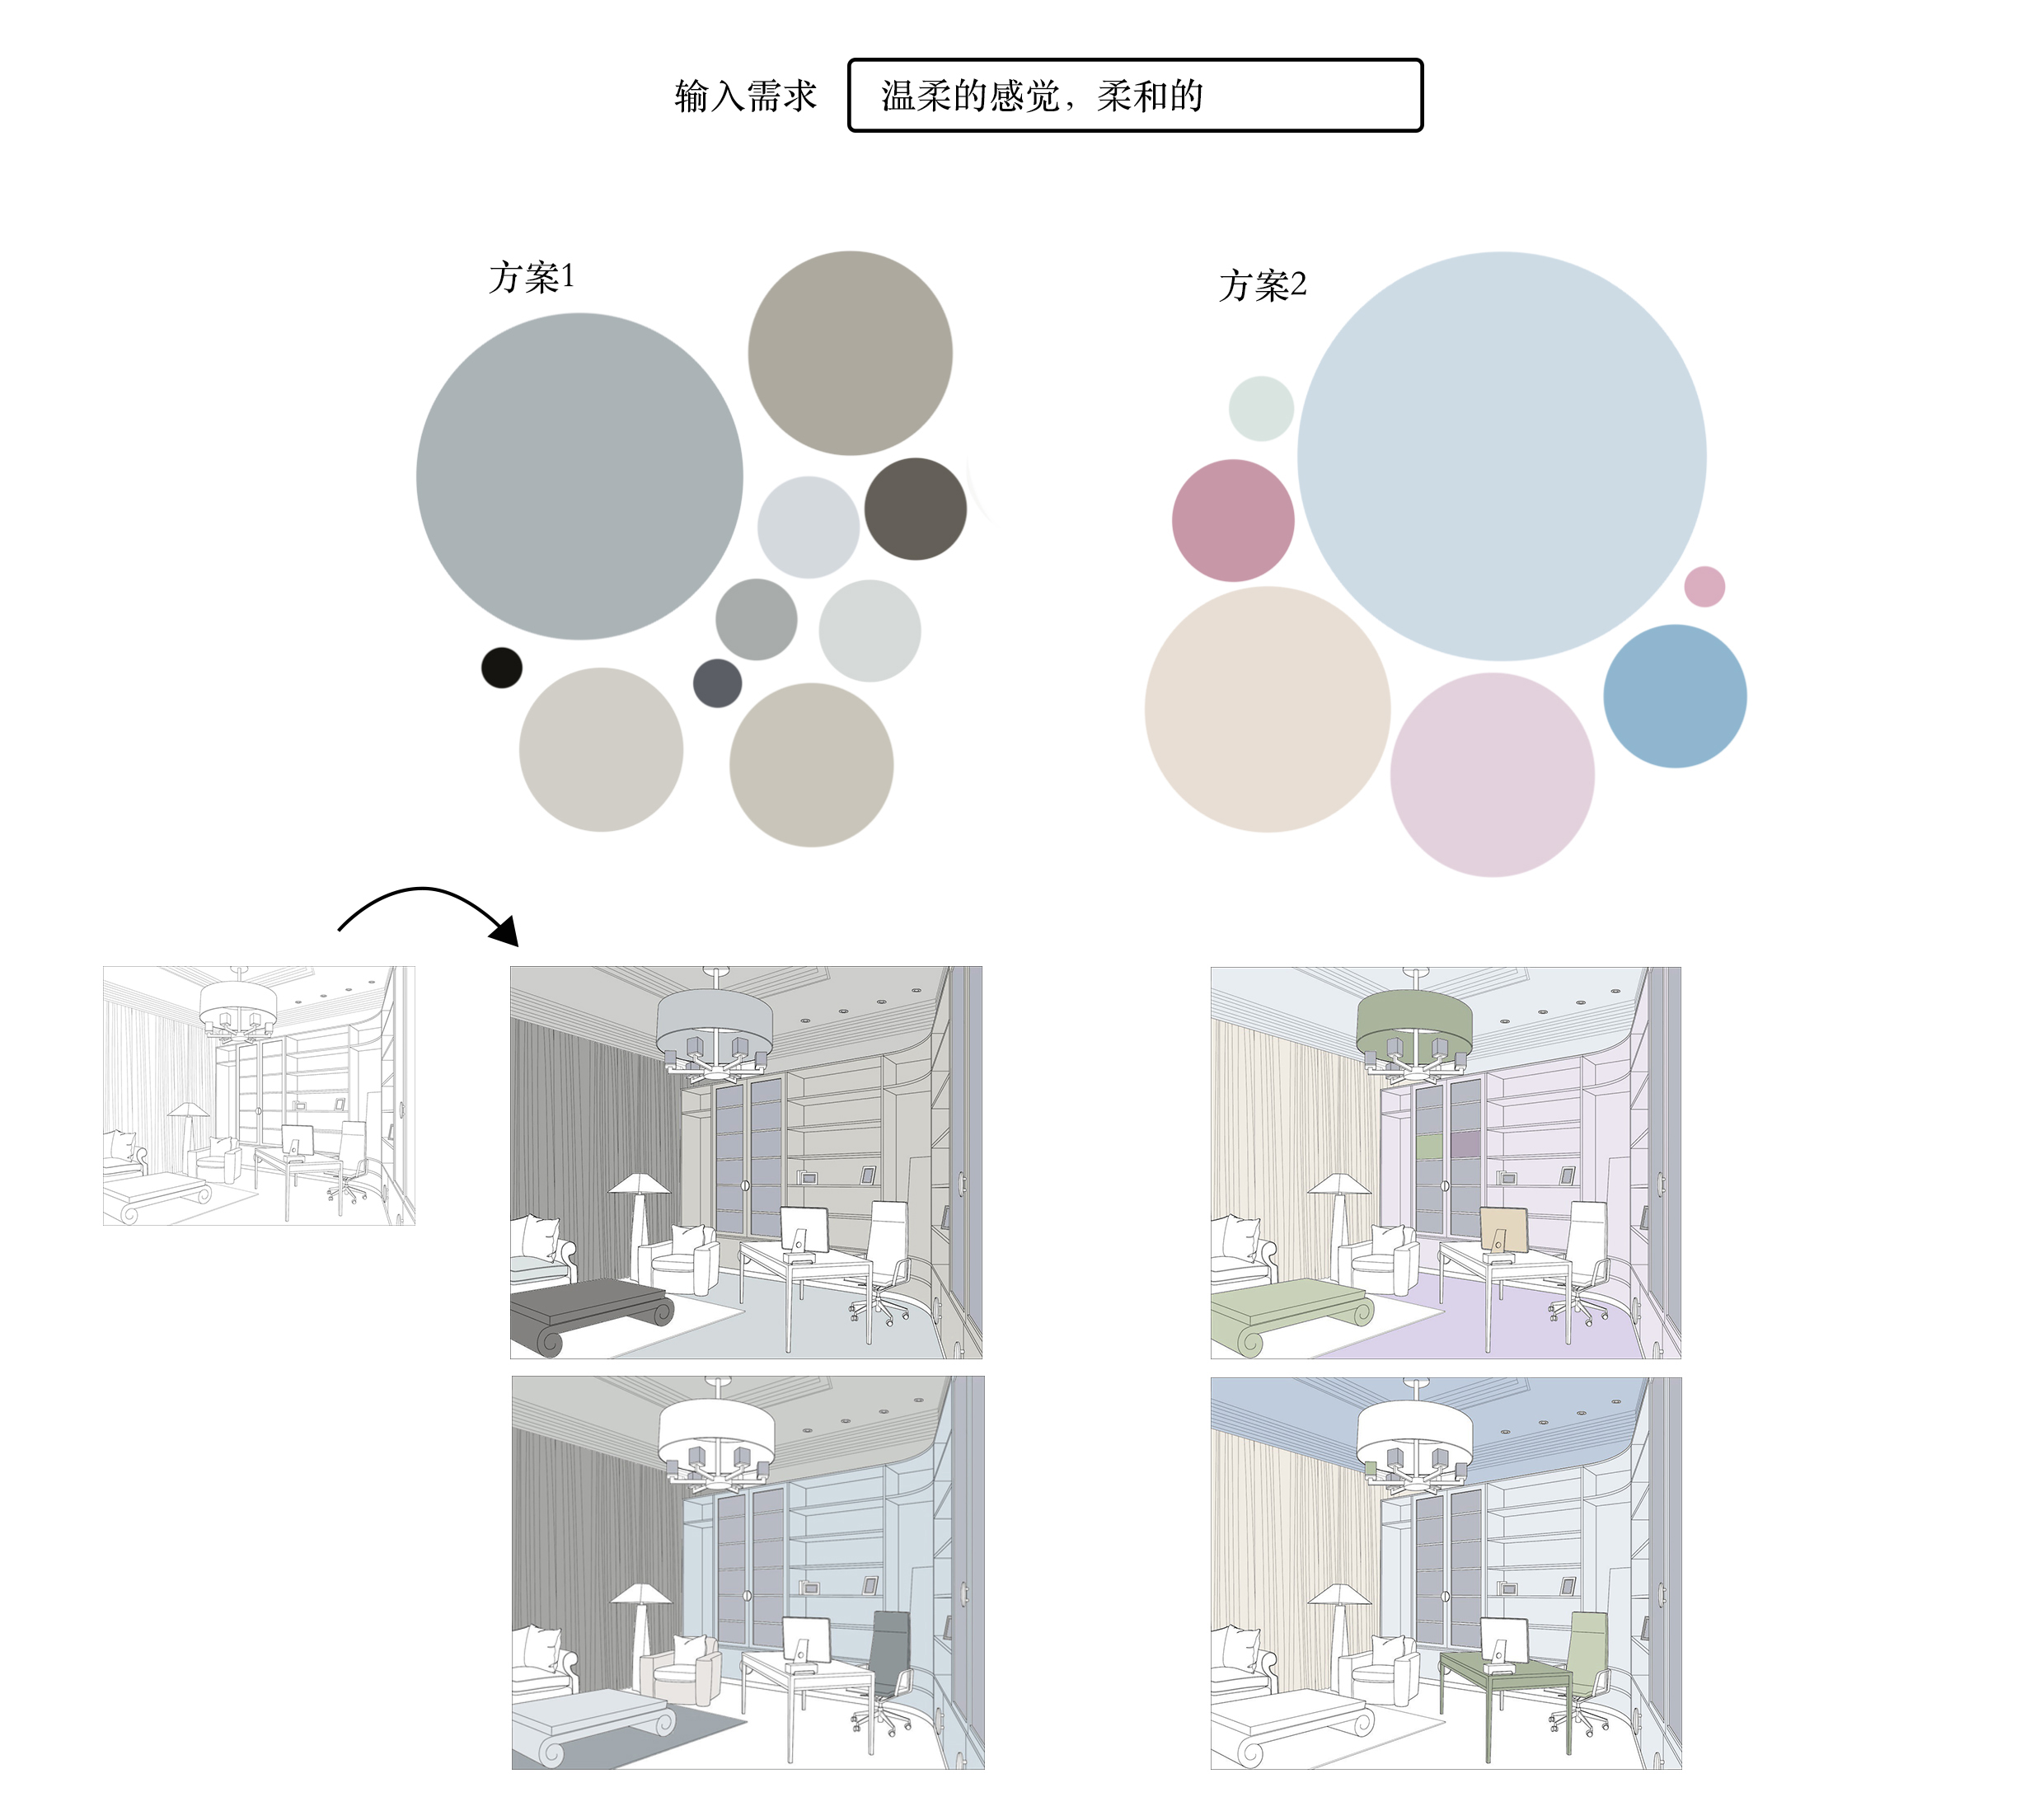
\includegraphics[width=\linewidth,keepaspectratio]{data/chapter-1/用户逻辑.jpg}
\caption{用户逻辑}
\label{figure:用户逻辑}
\end{figure}

搜索相匹配的艺术品这一步对用户来说是隐藏的,用户并不能看到相应的艺术品,而只得到色彩方案。这是为了让用户集中精力到他本来的任务中,关心配色方案而不用受到其他影响。输入设计需求的文本描述,就可以得到若干配色方案,并且可以每个配色方案都可以出现若干即时预览图,用户可以对各个配色方案有直接的感受。


\section{语义编码的实现}

\subsection{系统结构之语义搜索}

\begin{figure}[!htbp]
\centering
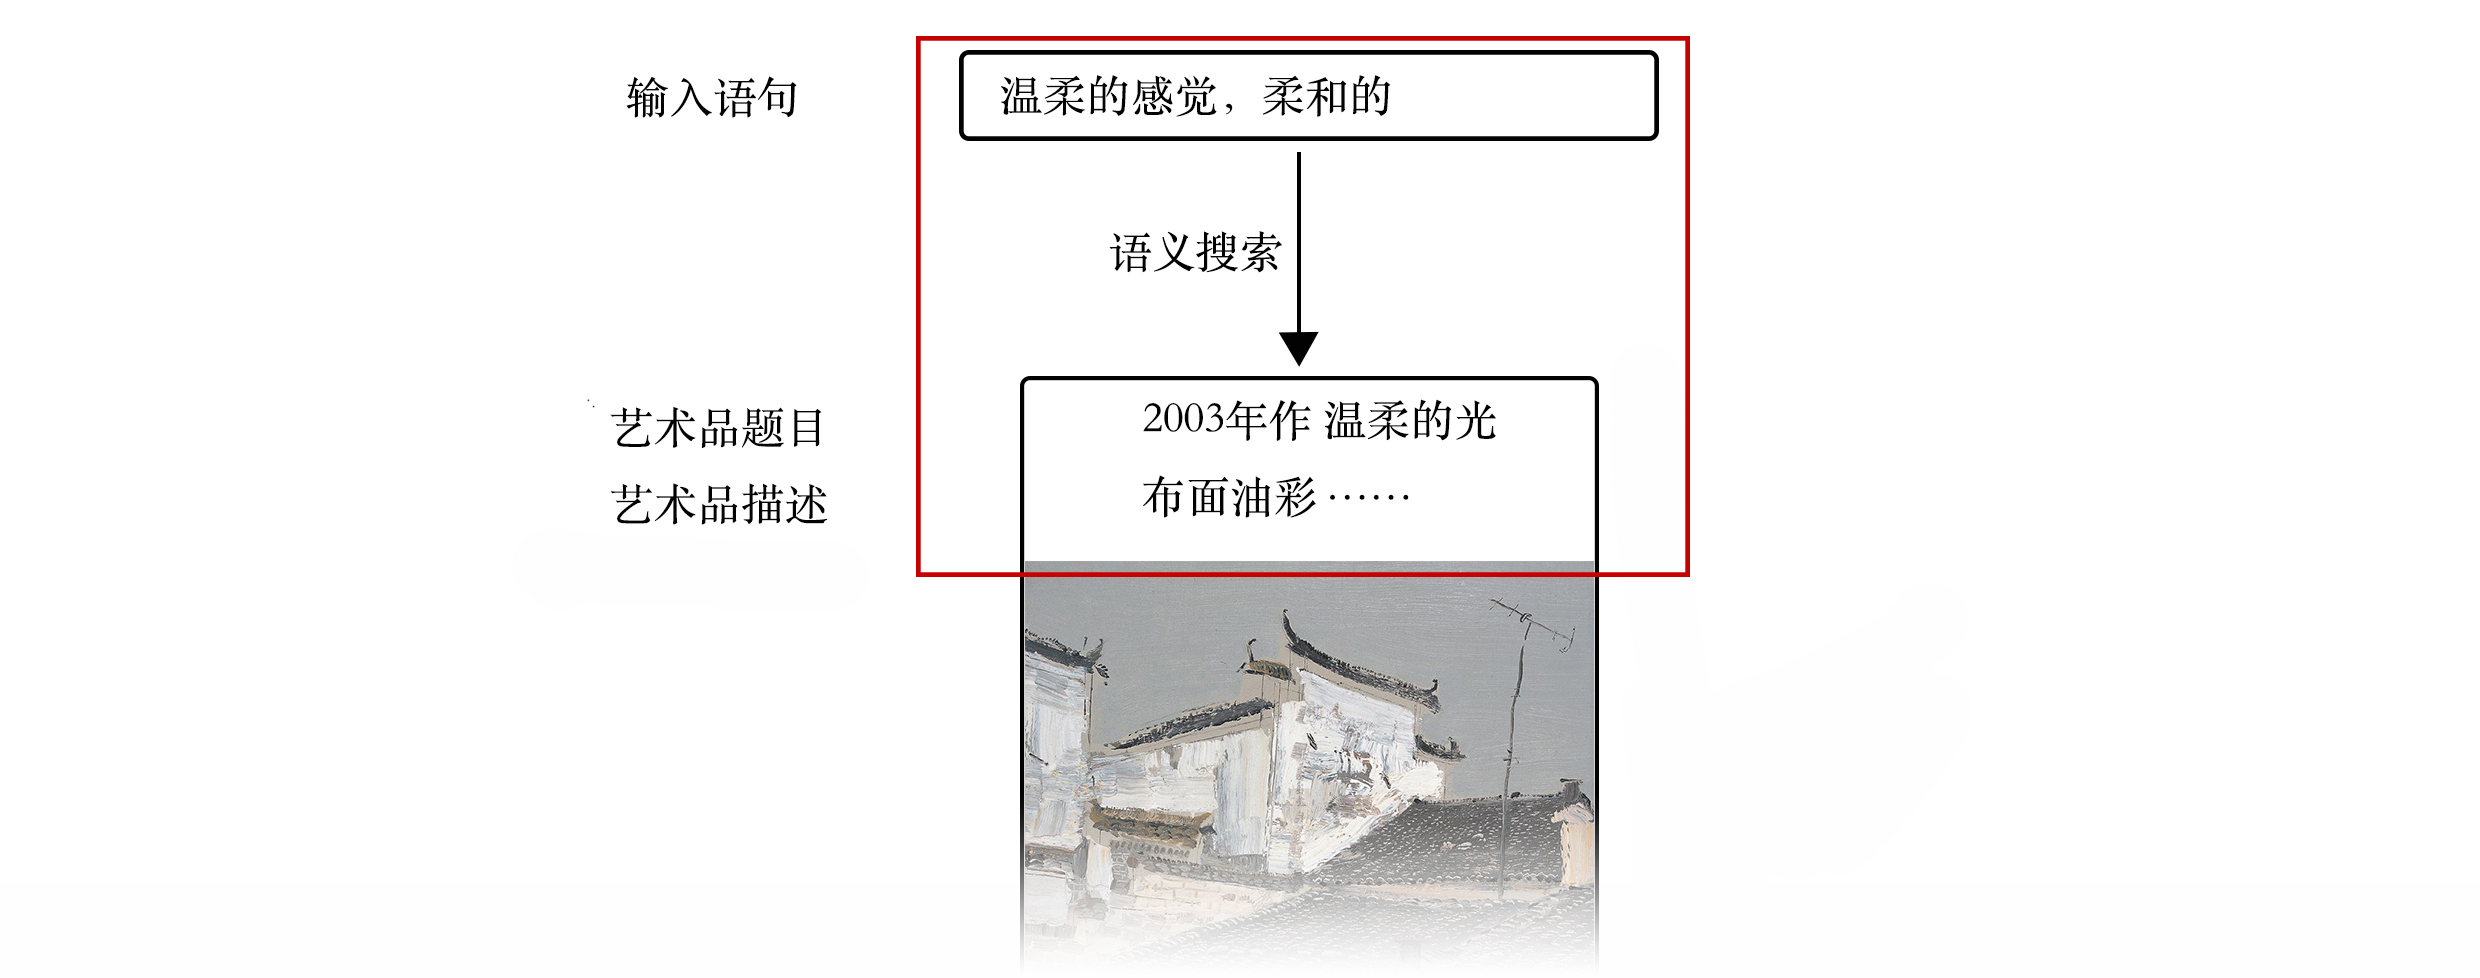
\includegraphics[width=\linewidth,keepaspectratio]{data/chapter-1/系统内部逻辑1步.jpg}
\caption{第一步:语义搜索}
\label{figure:语义搜索}
\end{figure}

图~\ref{figure:内部实现逻辑}中的第一步如上图~\ref{figure:语义搜索},就是搜索数据库中与用户输入相匹配的内容。要强调的是,我们的需求并非要提取关键词作为匹配,例如搜索含有某个词的字段,而是想做到搜索到词语意义相关的信息,例如输入“沮丧”可以匹配出“伤心,难过,忧伤的人”这样的字段,又例如输入“粉嫩”可以匹配出“少女”这样的字段。这就需要理解用户输入的内容和数据库中的文本内容,在其中作出意义上而非字面上的匹配。

\subsection{文本的向量化}

要使计算机理解文本的含义,从而进行搜索,对文本进行编码就需要满足以下三个要求:1.编码需要被计算机识别;2.编码需要包含单词的含义信息;3.所有的文本编码需要一定的整体同一性。

计算机理解文字的含义是困难的,即使计算机可以轻松的辨别出两句话是否一模一样,一句话中是否出现过某个单词,但是它却无法理解“苹果”和“梨”之间的关系(这对人类来说是常识),它也不能理解作为水果的“苹果”和“苹果”公司有什么不同(对于人类可以清楚的通过上下文理解这一点,不常混淆)。也就是说,文本的含义包括了语义,逻辑,上下文不同带来的多义。要用数字来表达这样复杂的信息,目前最好的解决方式是用向量来表达。

单词向量化是指将单词编码为向量形式,单词的向量化有多种方法,最简单的一种就是one-hot的向量。\cite{athier1997process}我们用一句话来举例子:“我 喜欢 吃 苹果,而 他 喜欢 吃 梨子。”这个句子长度为7个不同的单词。我们可以用这样的向量给每个单词编码,每个单词就可以表现为一个7维的向量,如表~\ref{table:one-hot},每个单词的向量为单词下的一列,就可以将一段文本的信息完整的保存进一个矩阵。

\begin{table}[!htbp]
\caption{one-hot向量}
\label{table:one-hot}
\centering
\begin{tabular}{|c|c|c|c|c|c|c|c|c|c|}
\hline
  & 我 & 喜欢 & 吃 & 苹果 & 而 & 他 & 喜欢 & 吃 & 梨子 \\
\hline
我 & 1 & 0 & 0 & 0 & 0 & 0 & 0 & 0 & 0 \\
\hline
喜欢 & 0 & 1 & 0 & 0 & 0 & 0 & 1 & 0 & 0 \\
\hline
吃 & 0 & 0 & 1 & 0 & 0 & 0 & 0 & 1 & 0 \\
\hline
… &  &  &  &  &  &  &  &  &  \\
\hline
\end{tabular}
\end{table}

这样的方法,如果对于文本长度较大的情况,就需要很大的空间储存这些向量,比如一本上万个单词的书籍,就需要单词的维度上万,里面大多数的位置又都是0。并且,这种方式对于不同文本来说并没有同一性,对于同一个词,不同的文本中必须有不同的词向量。最不好的一点是,这些词向量很难表示词的含义,例如近义词的向量和同类词语的向量,根本没有规律可循。

\begin{table}[!htbp]
\caption{词频向量}
\label{table:frequency-vec}
\centering
\begin{tabular}{|c|c|c|c|c|c|c|c|}
\hline
句子 & 我 & 喜欢 & 吃 & 苹果 & 而 & 他 & 梨子 \\
\hline
我喜欢吃苹果而他喜欢吃梨子 & 1 & 2 & 2 & 1 & 1 & 1 & 1 \\
\hline
我喜欢吃苹果,梨子 & 1 & 1 & 1 & 1 & 0 & 0 & 1 \\
\hline
他喜欢吃吃吃 & 0 & 1 & 3 & 0 & 0 & 1 & 0 \\
\hline
\end{tabular}
\end{table}

为了减少向量的维度,增加矩阵的密集程度,出现了基于词频的单词向量化。以我们的例句为例“喜欢”,“吃”这两个单词出现了两次,其他单词出现了一次。词频向量就是基于此构成。如表~\ref{table:frequency-vec},例如一篇文章中有表中的三句话,则每个单词的向量为单词下的一列,每句的向量为句子右侧的一行。词频向量和one-hot向量相比,维度有所下降,使用空间更有效率。词频也会记录一些文本的信息,不同的文本中单词的词频会有区别。然而完全从句子对单词计数,对词序信息完全忽略,同样难以提取文字本身的含义。

在此基础上的tf-idf的向量化不仅仅量化一个单词在一段文本中的频率,还考虑到在所有文本中单词出现的情况,这样就可以表征出一个单词和某段文本的关系。\cite{xia2011improvement}$tfidf = tf(t,d)*idf(t,D)$,其中 $tf(t,d)$ (term frequency)表征单词t出现在文本d中的频率。它可以有多种形式,比如$tf(t,d)=f_td$,$f_td$表示单词t出现在文本d中次数;或者考虑到文本到长度$tf(t,d)= \frac{f_td}{n_{in document}}$,$n_{in document}$指文章总共的单词数,$tf(t,d)$即出现在文本中的频率;甚至也可以是布尔的,当文本d中出现词t则 $tf(t,d)=1$ 否则$tf(t,d)=0$,等等。idf(inverse document frequency)定义为$idf(t,D) = log\frac{N}{n_{t occurs}}$ ,$N$表示总的文档数,$n_{t occurs}$表示含有单词t的文档数。

以之前的三句话为例:(a)我 喜欢 吃 苹果 而 他 喜欢 吃 梨子。(b)我 喜欢 吃 苹果。(c)我 喜欢 吃 吃 吃。则对于单词“我”,有:$tf(“I”,a)= \frac{1}{9}$,$tf(“I”,b)= \frac{1}{4}$,那么句子b中“我”这个词占整体比例更高。但对于所有文本,$idf(“I”,D) = log\frac{3}{3} = 0$,每个句子都出现了“我”这个词,所以$tfidf(“I”,a) = tfidf(“I”,b) = 0$。处理文档大量时,对于一些非常常见的词,比如“那个”“这个”这样的词,可以认为它们没什么意义,就会出现这种情况。而比如对于单词“苹果”,$tf(“apple”,a)= \frac{1}{9}$,$tf(“apple”,b)= \frac{1}{4}$,$idf(“apple”,D) = log\frac{3}{2} $,就会出现$tfidf(“apple”,a) = 0.045$,$tfidf(“apple”,b) = 0.1$。我以这三个句子计算了单词“我”和单词“苹果”的向量如表~\ref{table:tfidf-vec}:

\begin{table}[!htbp]
\caption{tfidf向量}
\label{table:tfidf-vec}
\centering
\begin{tabular}{|c|c|c|c|}
\hline
句子 & 我喜欢吃苹果而他喜欢吃梨子 & 我喜欢吃苹果 & 我喜欢吃吃吃  \\
\hline
我 & 0 & 0 & 0  \\
\hline
苹果 & 0.045 & 0.1 & 0 \\
\hline
… &  &  &  \\
\hline
\end{tabular}
\end{table}

只要有足够量的文本,tf-idf向量可以在文本间做比较,然而还有一个问题没有解决,那就是它仍然不包含单词语义的信息。在构建tf-idf向量的过程中,只用到了文本中单词的数量,完全没有使用单词的顺序信息,而文本中单词顺序所含有的信息是很重要的,如何将这些信息提取出来呢。

如果我们考虑上下文构建向量。对于句子“我 喜欢 吃 苹果 而 他 喜欢 吃 梨子”。将每个词前后对它有影响的单词数量,称为上下文窗口大小(context window)。比如,对于单词“喜欢”,在窗口大小为3时,单词“吃”在它周围出现的次数共2次,“我”、“苹果”、“他”、“梨子”、“而”各一次。如表~\ref{table:context}:

\begin{table}[!htbp]
\caption{上下文向量}
\label{table:context}
\centering
\begin{tabular}{|c|c|c|c|c|c|c|c|}
\hline
句子 & 我 & 喜欢 & 吃 & 苹果 & 而 & 他 & 梨子 \\
\hline
我   & 0 & 1 & 1 & 1 & 0 & 0 & 0 \\
\hline
喜欢 & 1 & 0 & 2 & 2 & 2 & 1 & 1 \\
\hline
吃   & 1 & 2 & 0 & 1 & 2 & 2 & 1 \\
\hline
苹果 & 1 & 2 & 1 & 0 & 1 & 1 & 0 \\
\hline
而   & 0 & 2 & 2 & 1 & 0 & 1 & 1 \\
\hline
他   & 0 & 1 & 2 & 1 & 1 & 0 & 1 \\
\hline
梨子 & 0 & 1 & 1 & 0 & 1 & 1 & 0 \\
\hline
\end{tabular}
\end{table}

在此基础上,如果我们采用一点统计学和数学的知识,使用神经网络的算法,就可以从文本中提取出更多的信息。word2vect就是这样一种算法,虽然前面所述都是单词向量化都方法,但word2vect被 Mitolov 等引入到自然语言领域之后,向量前所未有的拥有了密集的信息。对于一个出现在文本中的单词,在知道周围的词语的情况下,就能够预测出这个单词是某个单词的可能性。\cite{baroni2014don}比如“我喜欢吃(a)”,a是单词“苹果”的可能性就比a是单词“因为”的可能性更高。在非常大量文本的情况下,“苹果”和“梨子”常常出现在相似的环境下,算法就将计算得到它们的向量是相似的,从而被归为相似的词语。\cite{DBLP:journals/corr/abs-1301-3781}

word2vect由CBOW(Continuous bag of words) 和 Skip-gram model 两个部分共同组成。\cite{DBLP:journals/corr/abs-1708-00107}CBOW的工作方式为以全文训练神经网络,以求输入神经网络一个单词,输出他周围的一个单词。以one-hot向量编码的句子“我 喜欢 吃 苹果 而 他 喜欢 吃 梨子”作为例子,则全文的矩阵如表~\ref{table:one-hot},对于其中“喜欢”这个单词,则具体为假如输入“喜欢”的向量,则期望输出“吃”的向量。\cite{Mikolov:2013:DRW:2999792.2999959}

\begin{table}[!htbp]
\caption{输入}
\label{table:cbow-input}
\centering
\begin{tabular}{|c|c|c|c|c|c|c|c|c|c|}
\hline
喜欢 & 0 & 1 & 0 & 0 & 0 & 0 & 1 & 0 & 0 \\
\hline
\end{tabular}
\end{table}

\begin{table}[!htbp]
\caption{输出}
\label{table:cbow-output}
\centering
\begin{tabular}{|c|c|c|c|c|c|c|c|c|c|}
\hline
吃 & 0 & 0 & 1 & 0 & 0 & 0 & 0 & 1 & 0 \\
\hline
\end{tabular}
\end{table}

CBOW算法结构如图~\ref{figure:CBOW网络结构},假如输入“喜欢”的向量 $(0,1,0,0,0,0,0)$,则期望输出“吃”的向量$(0,0,1,0,0,0,0)$。输入为${1}\times{V}$的矩阵(在这里V为7),隐藏—输入层为${V}\times{N}$的矩阵,隐藏—输出层为${N}\times{V}$。N就是我们选择的最终得到的词向量的维度。输入为${V}\times{1}$的矩阵,这个矩阵的每个位置对应的是one-hot编码中该位置单词出现的概率。在层与层之间没有激活函数,而是线性函数。使用计算出的输出值和期望的输出值之间的误差作为loss函数,反向传播适应得到维度为N的权重$\vec{W}$。与此同时,单词"吃"对应的输入还有“苹果”或“梨”,或者在窗口大小更大时的其他单词。多个权重平均的向量就是单词“吃”的向量。

\begin{figure}[!htbp]
\centering
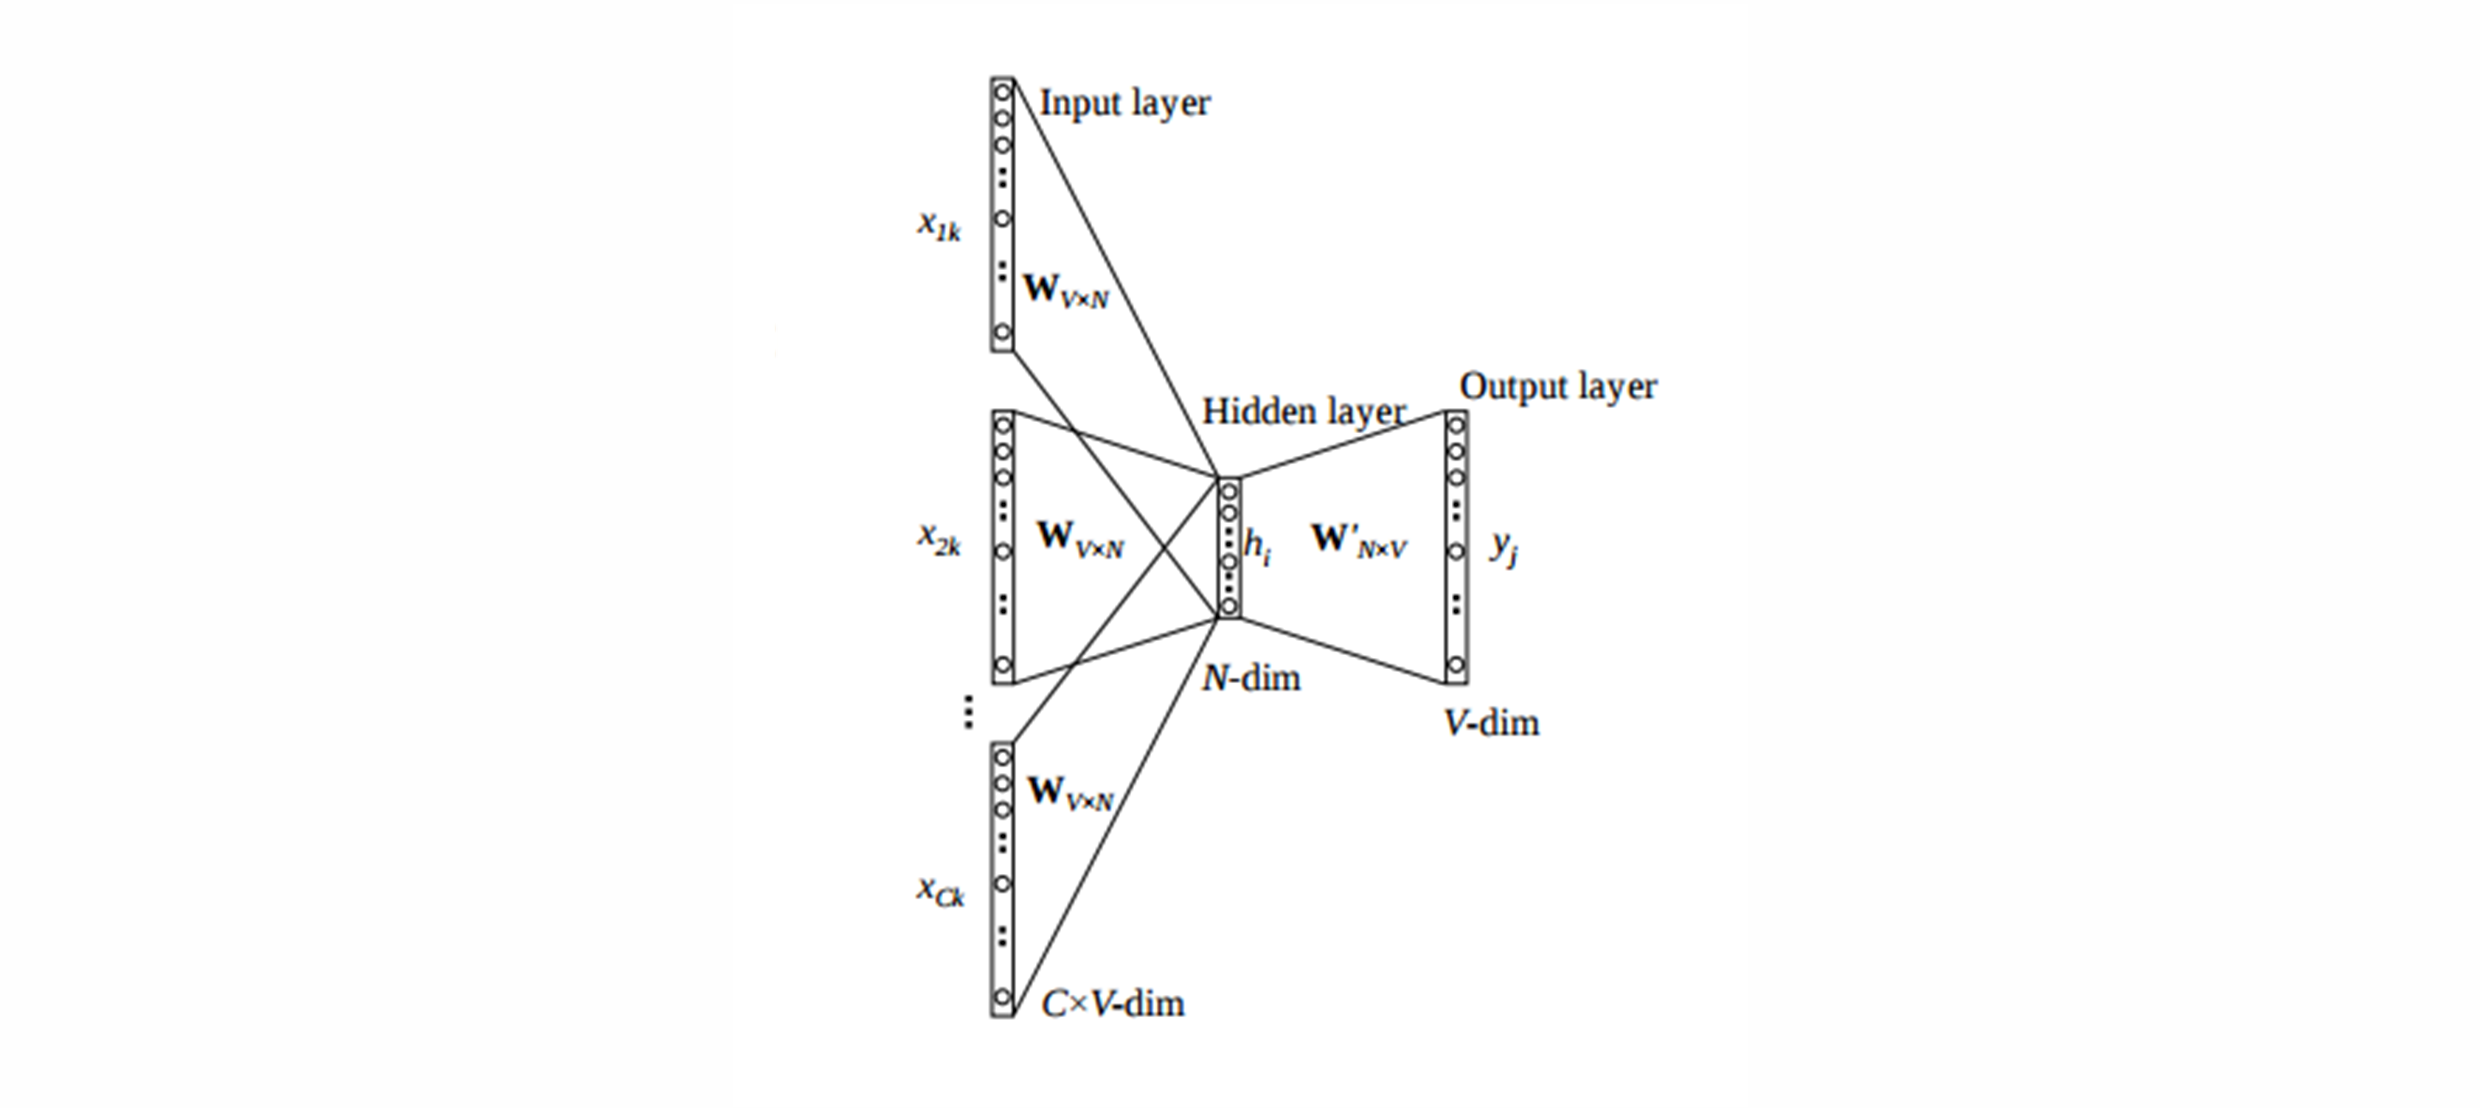
\includegraphics[width=\linewidth,keepaspectratio]{data/chapter-1/Screenshot-from-2017-06-04-22-05-44.png}
\caption{CBOW model}
\label{figure:CBOW网络结构}
\end{figure}

而Skip-gram model与之相似,只是输入的单词“喜欢”对应的输出有“我”,“他”,或者在窗口大小更大时的其他单词。对于多个输出单词就有多个误差向量,多个误差向量构成总的误差向量,反向传播适应得到维度为N的权重$\vec{W}$,即为单词“喜欢”的向量。

\begin{figure}[!htbp]
\centering
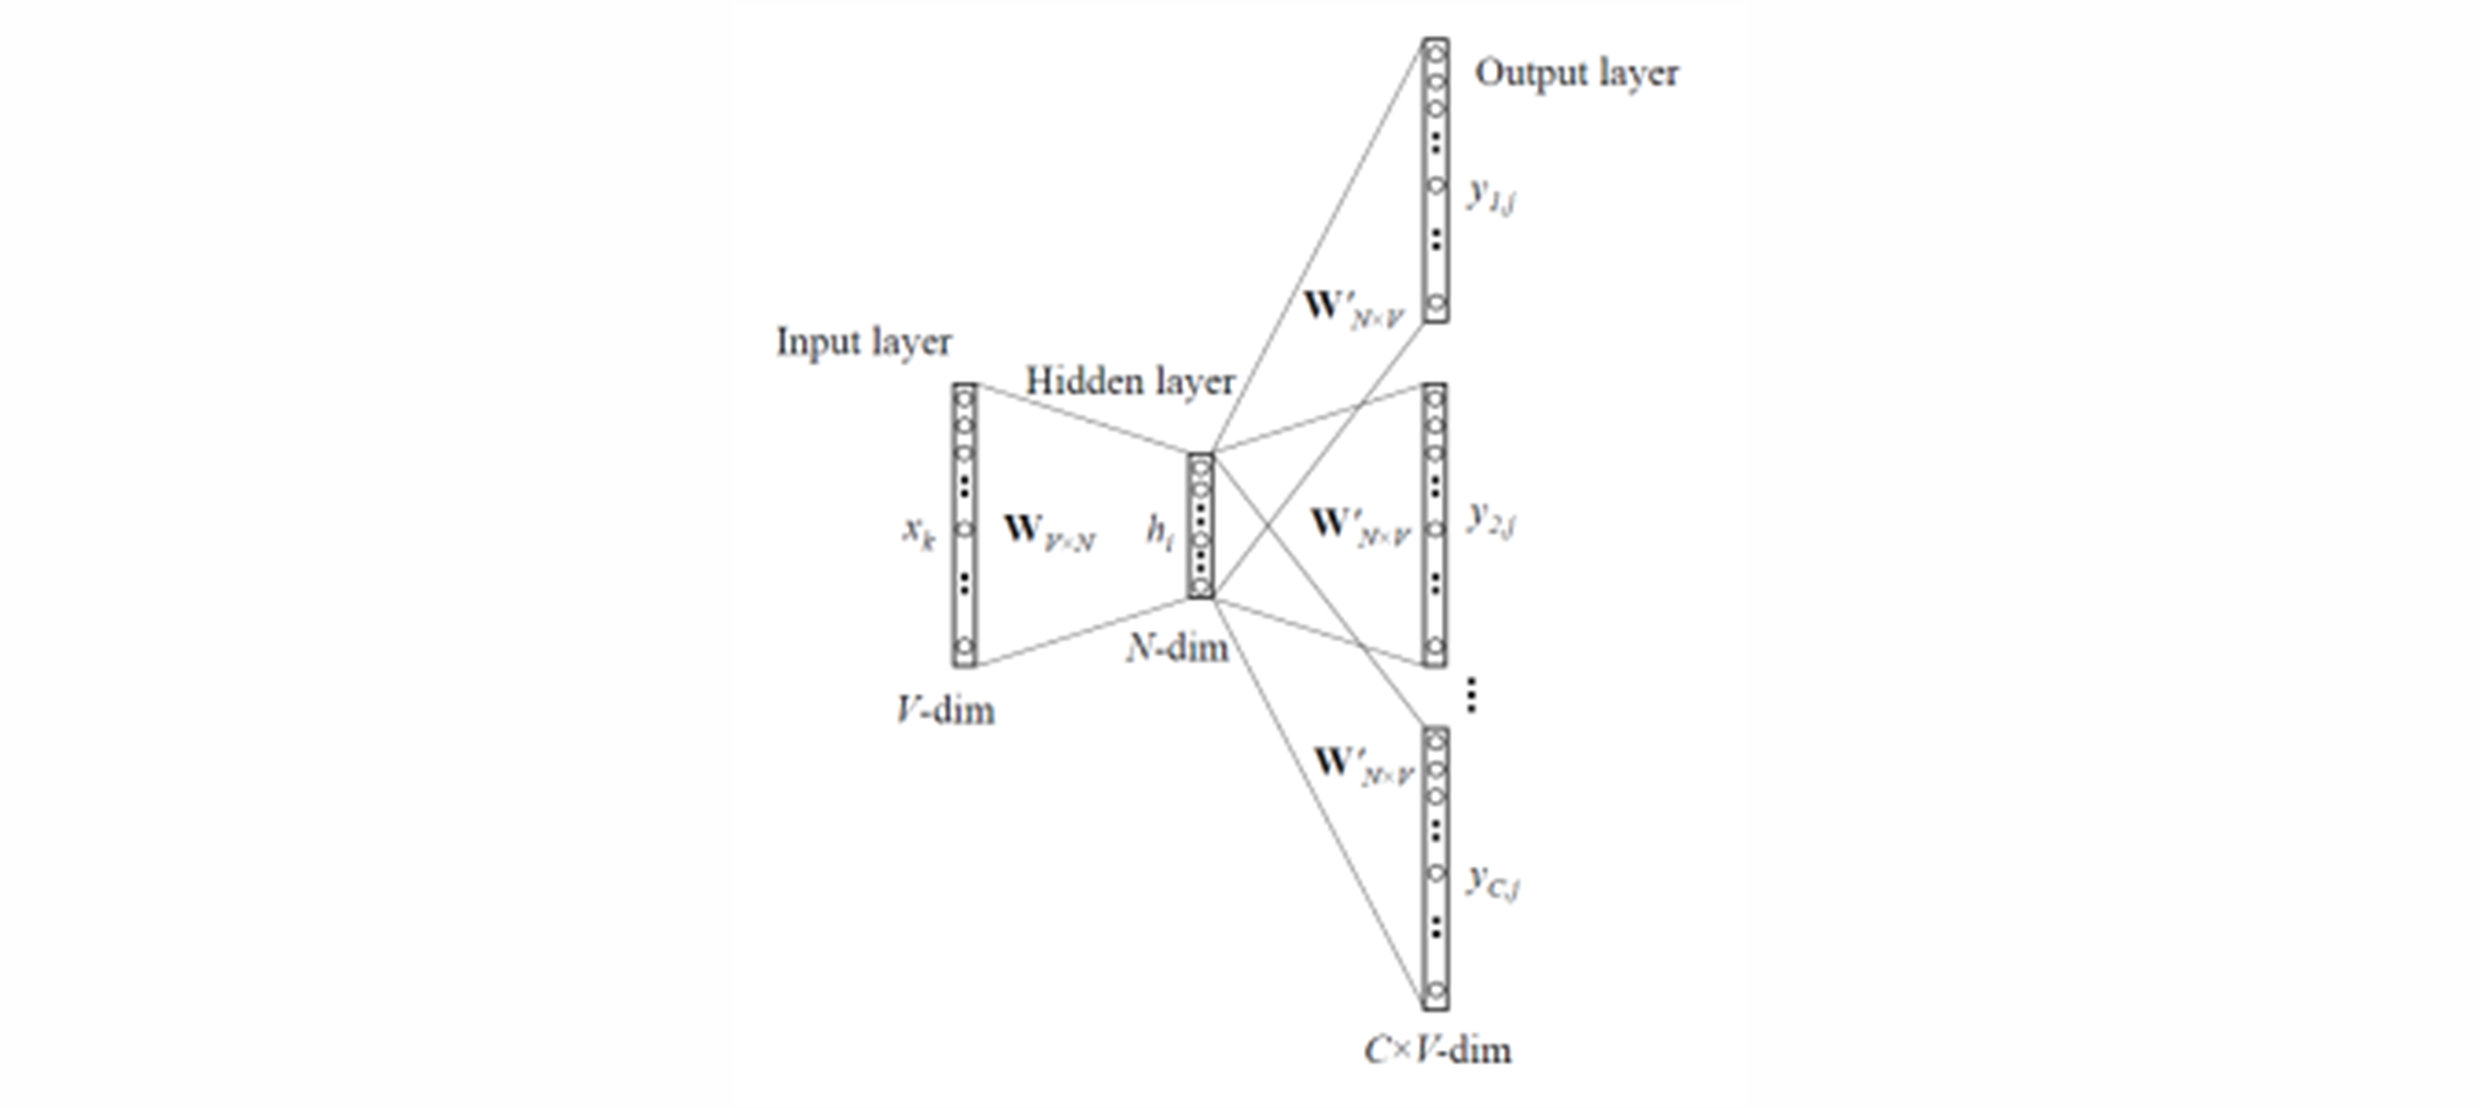
\includegraphics[width=\linewidth,keepaspectratio]{data/chapter-1/Capture2-276x300.png}
\caption{Skip-gram model}
\label{figure:Skip-gram网络结构}
\end{figure}

这种充分采用文字顺序的算法拥有很多很好的特性。比如,向量距离接近的单词意义也接近。更神奇的是,在训练文本多且全面的情况下,代表“女人”的向量和代表“妈妈”的向量之间的距离,与代表“男人”的向量和代表“爸爸”的向量之间的距离相等,即“女人”-“妈妈”=“男人”-“爸爸”;“苹果”这个单词的向量,同时和“梨子”的向量以及“IBM”的向量距离相等;由于是从文字的顺序提取信息,所以对于各种语言该模型都适用,也说明了提取的信息是语义上的而不仅仅是文本上的。

\subsection{本系统的单词向量化}

在介绍本系统的单词向量化之前,先要介绍我所使用的训练数据,训练词向量的数据来自两个来源,1.维基百科全文;2.艺术品交易数据库中的文本信息。其中艺术品交易数据库中的文本信息包含以下几种:1.艺术品交易数据库中每个艺术品的文本信息(包括艺术品的题目、描述和介绍、类型等);2.艺术品交易数据库中的所有文章(包括艺术品相关的新闻报道、微信文章、评论文章、艺术家专访等相关文章)。艺术品交易数据库中的文本信息是对艺术这一话题的加强训练。而采用维基百科的原因是,如果没有维基百科数据库,则当输入艺术品数据库中不存在的日常用语时就无法理解。为了系统能够响应人自然场景下的语言,采用一个普适的文本数据是非常必要的。对文本进行繁简体转化、中文分词之后,就可以作为训练使用的文本。

这样的庞大数据带来了更好的文本语义理解,但是也带来了计算量的问题。使用CBOW模型对单词进行word2vec向量化的过程中,如果文本有10000个单词,那么隐藏—输入层和隐藏—输出层就会是 ${10000}\times{N}$和${N}\times{10000}$的矩阵,需要反向传播调整和适应其中的每个权重计算量将会非常大,而维基百科和艺术品交易数据库带来的词量更是远大于此,对于如此大的计算量需要采用哈夫曼树进行优化,从而可以利用Hierarchical Softmax加速。\cite{DBLP:journals/corr/abs-1801-09797}

\begin{figure}[!htbp]
\centering
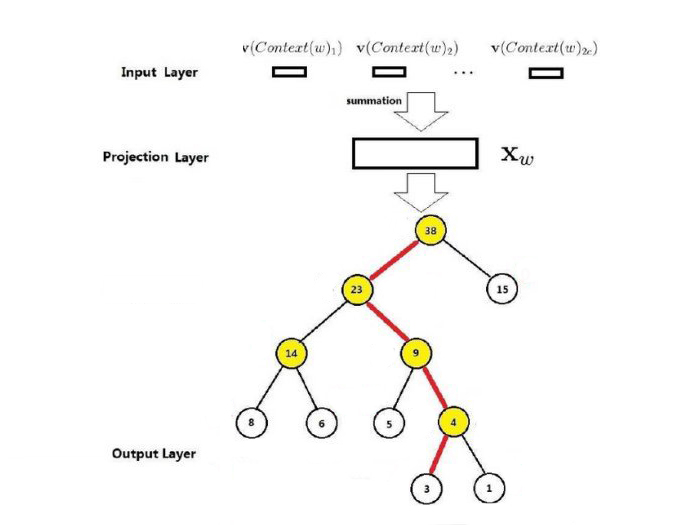
\includegraphics[width=\linewidth,keepaspectratio]{data/chapter-1/006iXRQMzy75IEZuWeoc4&690}
\caption{使用哈夫曼树的CBOW model}
\label{figure:使用哈夫曼树的CBOW model}
\end{figure}

哈夫曼树(Huffman Tree)又叫最优二叉树,是给定n个权值作为n个叶子结点,构造一棵二叉树,使得带权路径长度达到最小。哈夫曼树是带权路径长度最短的树,权值越大的结点离根越近。Skip-gram model的输出层使用哈夫曼树,总的文本中的每个词对应哈夫曼树中的一个叶子节点 (每个节点对应一个最后得到的word2vec词向量),每个非叶子节点定义一个向量(起到辅助的作用)。对于词典中的任意单词,哈夫曼树中必然存在唯一一条从根节点到该单词对应的路径,这样对于每一个单词,输出层只需要调整哈夫曼树路径上的向量。如果对于有V个单词的文本来说,本来隐藏—输入层和隐藏—输出层需要反向传播调整 ${V}\times{N}$和${N}\times{V}$个值,现在在哈夫曼树上每次二分产生一个概率,只需要经过log(V)次运算就得到了单词a出现的概率$p(a|context(a))$。

与此同时,本系统的word2vec还使用了以下的策略,把常见的词组作为一个新的单词增加到词典中,比如“苹果手机”;少采样常见的词,比如“而”“就”这些出现频率非常高的词其实它的表达的意思很少;采用Negative Sampling策略,通过负采样,每次修改其中一小部分weight,而不是全部。这些策略减少了训练的计算量,而且提升了最后word vector的质量。\cite{mikolov2013distributed}\cite{DBLP:journals/corr/abs-1301-3781}\cite{DBLP:journals/corr/abs-1801-10198}

CBOW模型实际上只考虑了单词有哪些上下文,而并未考虑单词的顺序,比如“我喜欢苹果”和“苹果喜欢我”在CBOW模型中的特征是一样的。加入了 N-gram 特征将“我-喜欢”和“喜欢-我”也加入单词的特征,也使用n-gram特征来将局部词序考虑在内,比如“女-朋友”“陶-瓷”。可以得到表达意义更准确的词向量。

使用上述的文本和模型训练维度为300的词向量,词典中包含全部文本中出现的单词。使用此词典构成输入语句和艺术品信息的语句向量。


\subsection{本系统的句向量建模}

在本系统中,需要语义搜索的内容并不是单词。输入语句是使用者输入的,不确定的语句,可能是一个或数个词语、短语、完整的或不完整的句子,总的说来,是一个或多个单词的序列,之后我们将其称为“输入语句”,即和我们平时口语采用的语言是相似的,不拘结构但求表达需求。而数据库中每个艺术品的文本信息由艺术品的题目、介绍,类型三个部分组成,短至一个词语(在文本信息只有一个单词的题目的时候),长至数段话(在文本信息包括大量描述和介绍的时候),总的来说也是一个或多个单词的序列,之后我们将其称为“艺术品语句”。需要从使用者输入的语句定位到某一件艺术品,那么就需要输入语句的含义,和某件艺术品语句的含义相匹配。

要提取一段语言的意义,就需要将这多个表达单词意义的向量转化为一个转化语句意思的向量。在这个将多个词向量加和为语句向量的过程,需要考虑这三点:

1.词汇的含义,语句由词汇构成,语句中词汇的意思对语句的含义是决定性的,比如一张油画的名字叫做“忧伤的河流”说的就是忧伤,不是喜悦,是河流,不是山川。

2.词汇的频率,在语句中词汇出现的频率会对语句的意义产生影响,这样的影响并非线性的,有时,频率高的词表达的含义反而少,比如“作者非常非常思念家乡”,中出现了两个“非常”,表达比“非常”更深的程度,但是句子主要要表达的意思仍然是“作者思念家乡”,这句话和“作者很思念家乡”的含义相似,而和“我非常非常喜欢吃苹果”是不同的;而有的时候频率高的单词直接是这段文本中的重要主题和中心。大概率的,总体文本中频率高的词带来的含义有限,这些词比如“有”“这”“那”,并不影响语句的意义,而总体文本中概率一般然而特定文本中频率高的词,比如在某个作品的描述中常常出现“热烈”“欢快”,往往对这一文本的语义的影响很大。

3.词汇的位置。词汇的位置有时也代表了词汇含义的重要性。语言是结构性的序列,在结构的某一位置上的词语往往代表更重要的含义。对于词语构成语句的过程,这个位置的重要性很灵活。比如对于语句“作者非常思念家乡”,如果这句话处在一个环境中,上一句话是“谁思念家乡了?”,那么最重要的位置就是主语的“作者”,而如果上一句话是“作者思念什么”,那么最重要的位置就是宾语“家乡”。另外,如果考虑句子构成完整段落的过程,段落的第一句话和最后一句话,由于可能是总起和总结的句子,所以格外重要,这也是考察位置得到的信息。

对单词向量直接加和求得输入语句的向量是最简单的方法,即$\vec{S}=\sum_{i=0}^{n}{w_i}$。其中$\vec{S}$指据向量,句子中有n个单词,${w_i}$指第i个单词的词向量。\cite{DBLP:journals/corr/abs-1801-10198}这种方法简单快捷,但是它只考虑了语句中词汇的含义,并没有考虑到词汇的频率和词汇的位置对句向量的影响。会导致语句中重复出现的词语对语句影响严重的情况,另外也会让一些本来并不代表意义的单词占比较大,比如对于语句“我要一个柔和一点的色彩方案”,这句话中“柔和”其实是最关注的一个词,但是由于干扰信息太多,如果直接加和,这句话的向量会和“我要一个欢快一点的色彩方案”更近,而与单词“柔和”并不相近。更突出的一个例子是,很多作品的题目中会出现作品的媒介比如“儿童 布面油画”,“温柔的风 油画”等等,其中,单词“布面”、”油画“等,它们在整体文本中大量出现,但对于每个作品已经有了明确的分类信息,文本信息中更多的是为了匹配作品的内容和色彩风格,它们就并非与作品色彩风格有关的单词。

在这种情况下,我采用了加权加和的方法,即$ \vec{S} =\sum_{i=0}^{n}{ \vec{w_i}}*{weight(w_i)}$ ,这样可以通过权重过滤掉干扰信息。\cite{DBLP:journals/corr/abs-1708-00107}\cite{DBLP:journals/corr/abs-1801-10198}我使用单词在总体文本中的词频作为权重分析的来源,在总体文本中出现频率越高的词就说明它是不重要的(如果一个单词出现在每一句话中,那么这个单词当对分辨每句话的意义并没有价值)。如此,则权重$ weight(w_i)=\frac{1}{frequency(w_i)}$ ,句向量的计算方式则为:

$$ \vec{S} =normalization(\sum_{i=0}^{n}{ \frac{\vec{w_i}}{frequency(w_i)}})$$

以词频的倒数为权重,对语句中的单词加权求和,再经过归一化,得到语句向量。对于输入语句如此即可求出其句向量,而对于艺术品语句则还要加上一个内容分类权重,由于艺术品语句的内容分为题目、介绍和类型,三者表达信息的权重是不同的,其中题目与艺术品本身的含义和特点最为联系紧密,而介绍有时详细描述了作品的风格和内容,有时却是和作品本身的内容关系不大的作者背景介绍等,在这样不稳定的情况下,我为系统设置了可调节的权值。

$$ \vec{S} =normalization(\sum_{i=0}^{n}{ \frac{\vec{w_i}}{frequency(w_i)}\times weight_{txt type}})$$

\subsection{搜索算法}

每一件艺术品都有独一无二的文本信息,也就是对应唯一的艺术品语句向量。计算出每件艺术品的艺术品语句向量,将每件艺术品的向量储存在艺术品“词典”,输入语句向量在词典中搜索,找到最匹配的艺术品语句向量,即可定位到最匹配的艺术品。取最符合得到前10件艺术品作为备选,可以包容更多的使用情况,这些情况的具体细节在下一小节“色彩提取”中将会详细描述。\cite{zhang2009vector}

\begin{figure}[!htbp]
\centering
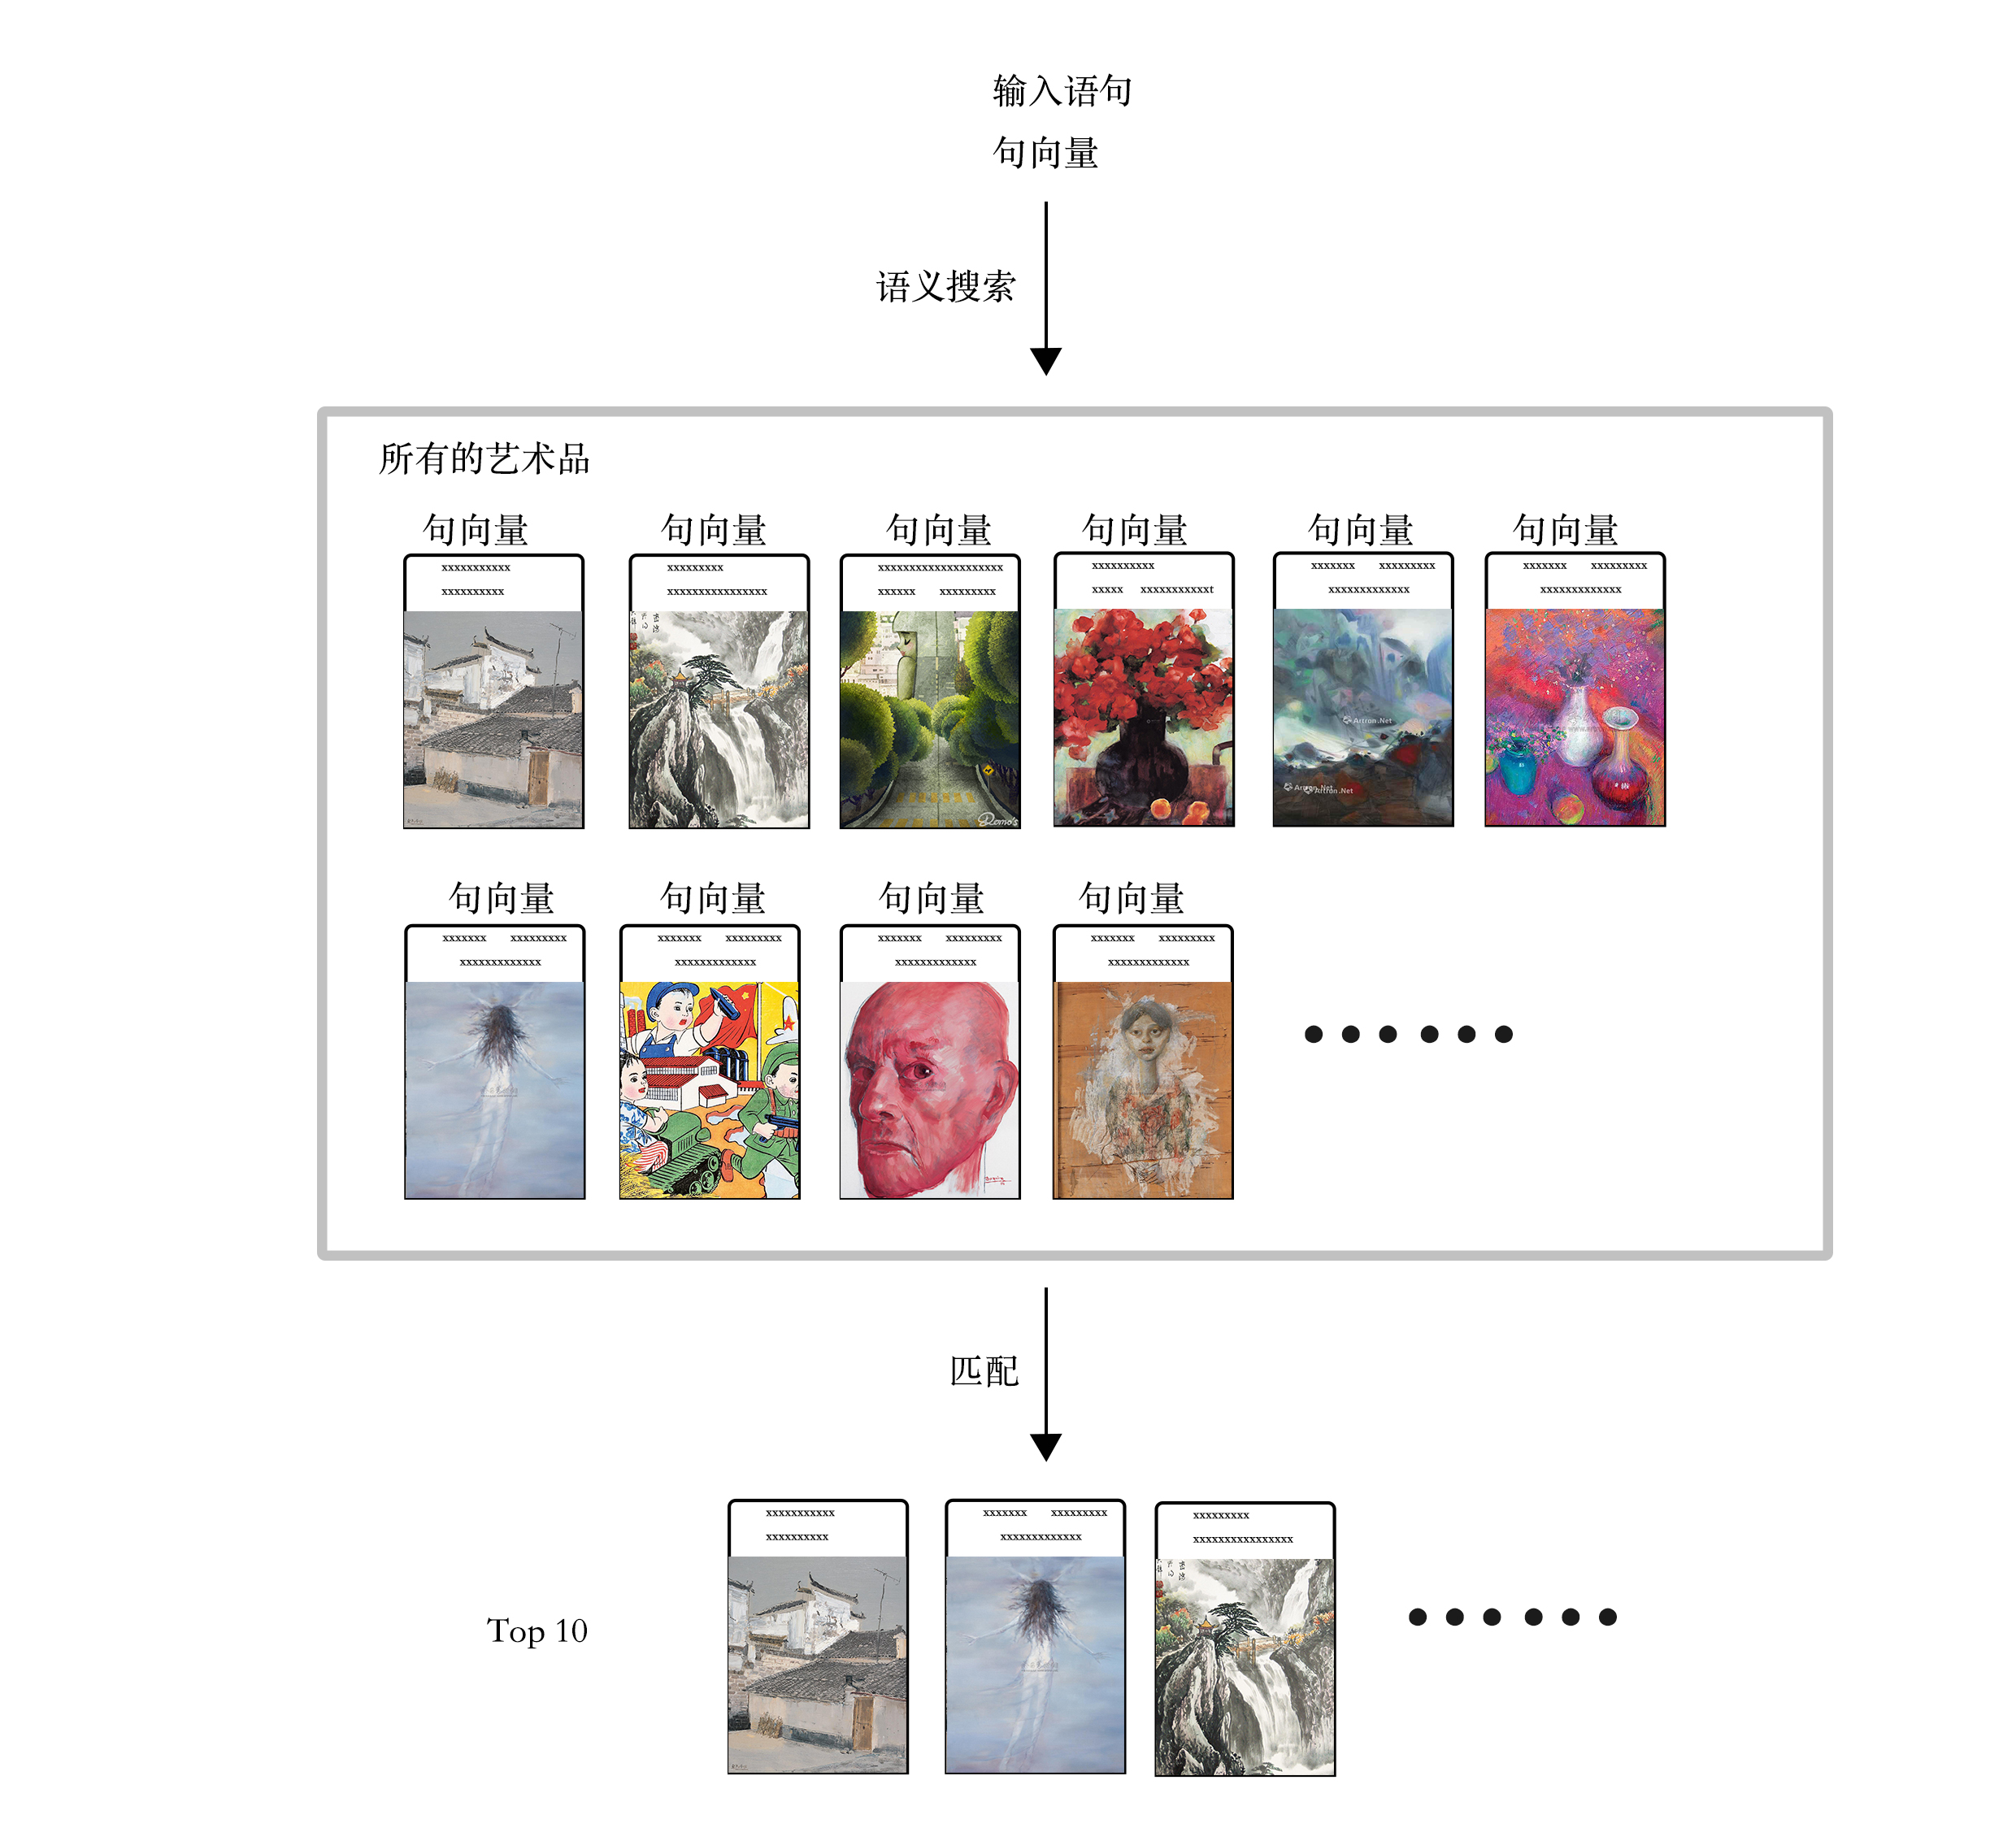
\includegraphics[width=\linewidth,keepaspectratio]{data/chapter-1/搜索.jpg}
\caption{匹配范围}
\label{figure:搜索}
\end{figure}

表征向量的相似度使用余弦相似度。词向量和句向量都经过归一化,向量指向同一方向即为匹配,也就是说向量之间的距离大小即为夹角的大小。如图~\ref{figure:余弦相似度}当两个向量指向相同,余弦为1,两个向量正交,余弦为0,指向相反余弦则为-1。两个向量夹角的余弦值可以确定两个向量是否大致指向相同的方向,故而考量输入向量与艺术品向量的距离使用余弦相似度。\cite{DBLP:journals/corr/abs-1802-09914}

\begin{figure}[!htbp]
\centering
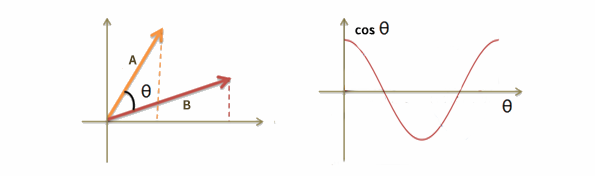
\includegraphics[width=\linewidth,keepaspectratio]{data/chapter-1/1-1.png}
\caption{余弦相似度}
\label{figure:余弦相似度}
\end{figure}

余弦相似度不仅对于二维向量适用,对于任何空间中度向量都适用。

$$ similarity = cos(\theta)= \frac{\vec{A}\cdot\vec{B}}{\|A\| \cdot \|B\|} = \frac{\sum_{i=0}^{n}{A_i \times B_i}}{\sqrt{\sum{{A_i}^2}} \times \sqrt{\sum{{B_i}^2}}}$$

本系统中的词向量和句向量维度为三百,对于归一化之后的句向量来说,所有的句向量的模都是1,即$\|A\| = \|B\|=1$,则

$$ similarity = cos(\theta)=  \sum_{i=0}^{300}{A_i \times B_i} = \mathbf{A} \times \mathbf{B^T}$$

对输入语句的句向量与每个艺术品语句的句向量做矩阵乘法,结果最接近1的就是最匹配的艺术品语句向量,此艺术品的语句和输入语句在语义上是最接近的,由此决定此艺术品就是与输入的语句最匹配的艺术品。\cite{ravichandran2005randomized}接下来就从这个艺术品来提取特征。

在本系统中还为了特定的需求进行一些搜索优化。由于本系统最终是为了从艺术品提取色彩,所以降低色彩很少的作品被搜索到的概率。比如对于书法作品,一般并没有色彩可以用于提取。搜索概率高的艺术类型设置为摄影、综合媒材、水粉水彩、油画、版画,以绘画作品为主。

由于艺术品和文字表达的模糊性,有时文字信息匹配度最高度艺术品事实上并不完全匹配,这种情况的出现往往是由于艺术家为了某些内涵,让艺术品的命名与艺术品内容表面上并不相关,或者艺术品的介绍过于偏重作者的家世、背景,与艺术品的内容关联度很低。为了解决这样的问题,在匹配的过程中,输入语句后,本系统取相似度前10的艺术品作为候选,随机选定其中一件作品提取色彩,当用户不满意当前匹配的色彩可以通过重复点击进行切换,用户也可以选择进入页面进行选择。

\section{色彩提取}

\subsection{系统结构之色彩提取}

由于艺术品的图片和文本语义信息的关联,艺术品图像风格的偏序特性保持到语义描述的偏序特性中,当输入语句和艺术品语句匹配成功后,自然就得到了与输入语句匹配的艺术品的图像。从艺术品图像中提取色彩特征,就可以得到相匹配的色彩方案。

\begin{figure}[!htbp]
\centering
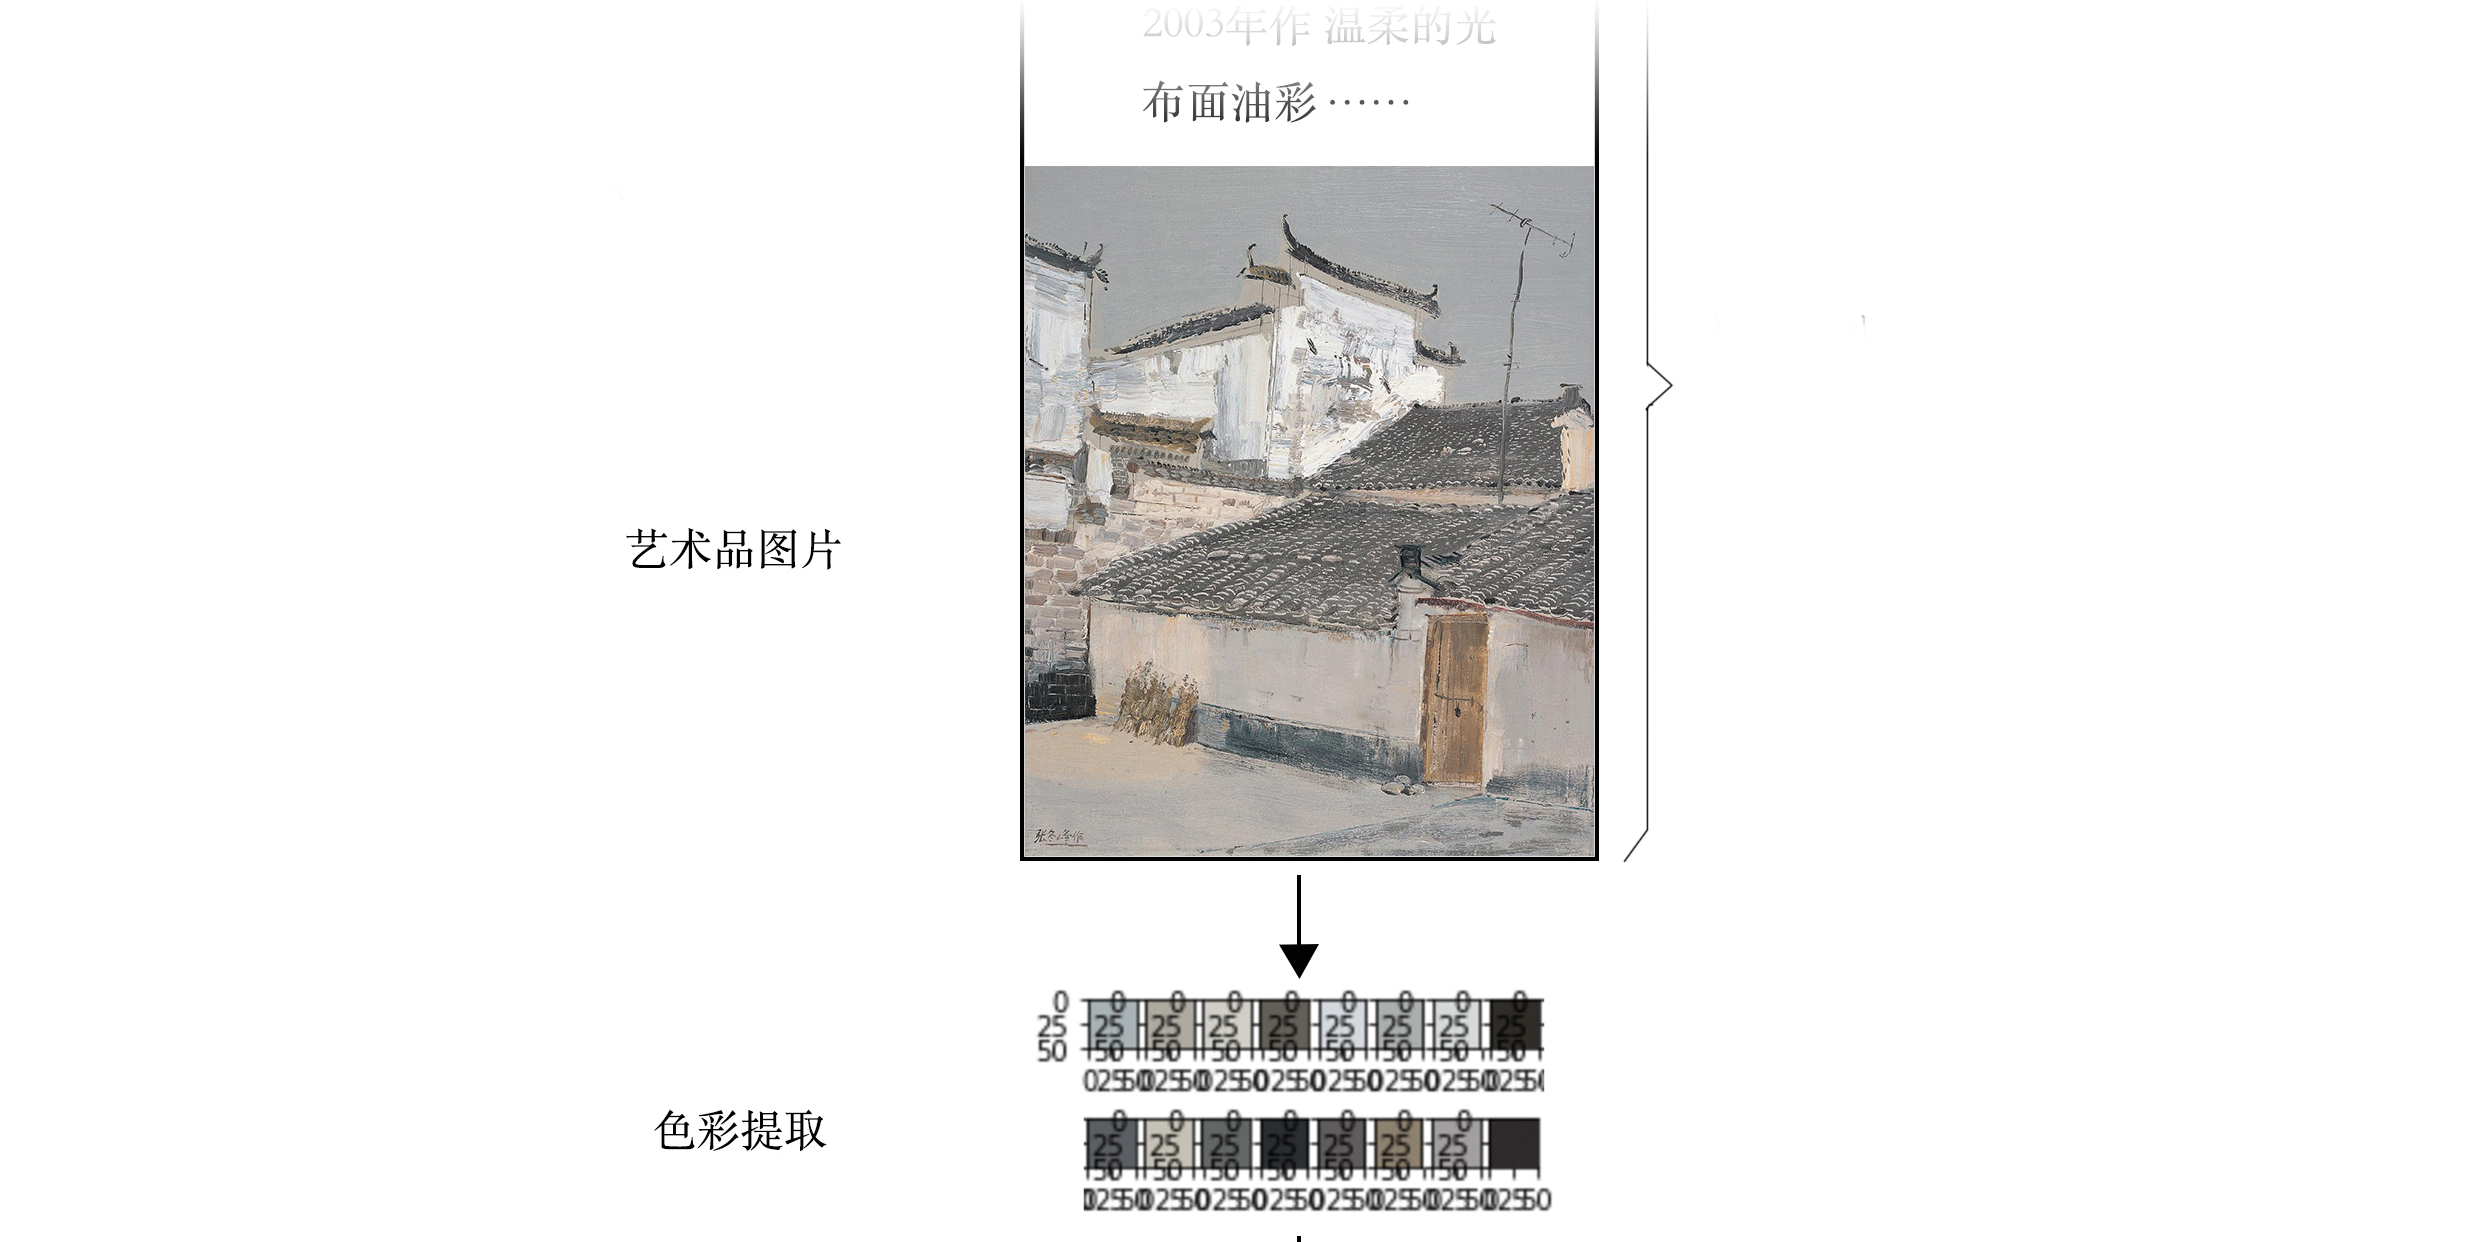
\includegraphics[width=\linewidth,keepaspectratio]{data/chapter-1/系统内部逻辑提取.jpg}
\caption{第二步:提取色彩}
\label{figure:系统内部逻辑提取}
\end{figure}

这一步输出的色彩方案使用RGB色彩模式,每个颜色包括Red-Green-Blue三个通道的值和该颜色本来在艺术品中占的比例(面积比例)。从艺术品图片中占比例最大的颜色开始,可以自定义提取颜色的个数,在本文的测试中取颜色的个数为16。

对于用户来说,输入文本并搜索将会出现一组色彩方案,这个色彩方案来自文本相似度与输入文本排前10的艺术品之一,用户可以通过不改变输入文本,再次搜索,从相似度前10的艺术品中另外随机选择一件,也可以直接打开相似度前10的所有色彩方案手动选择。如图~\ref{figure:搜索结果}虚线框中为文本相似度与输入文本排前10的艺术品,这些内容不展示给用户,用户仅仅关注色彩方案,通过重新搜索,或进入10个色彩方案可以选择。

\begin{figure}[!htbp]
\centering
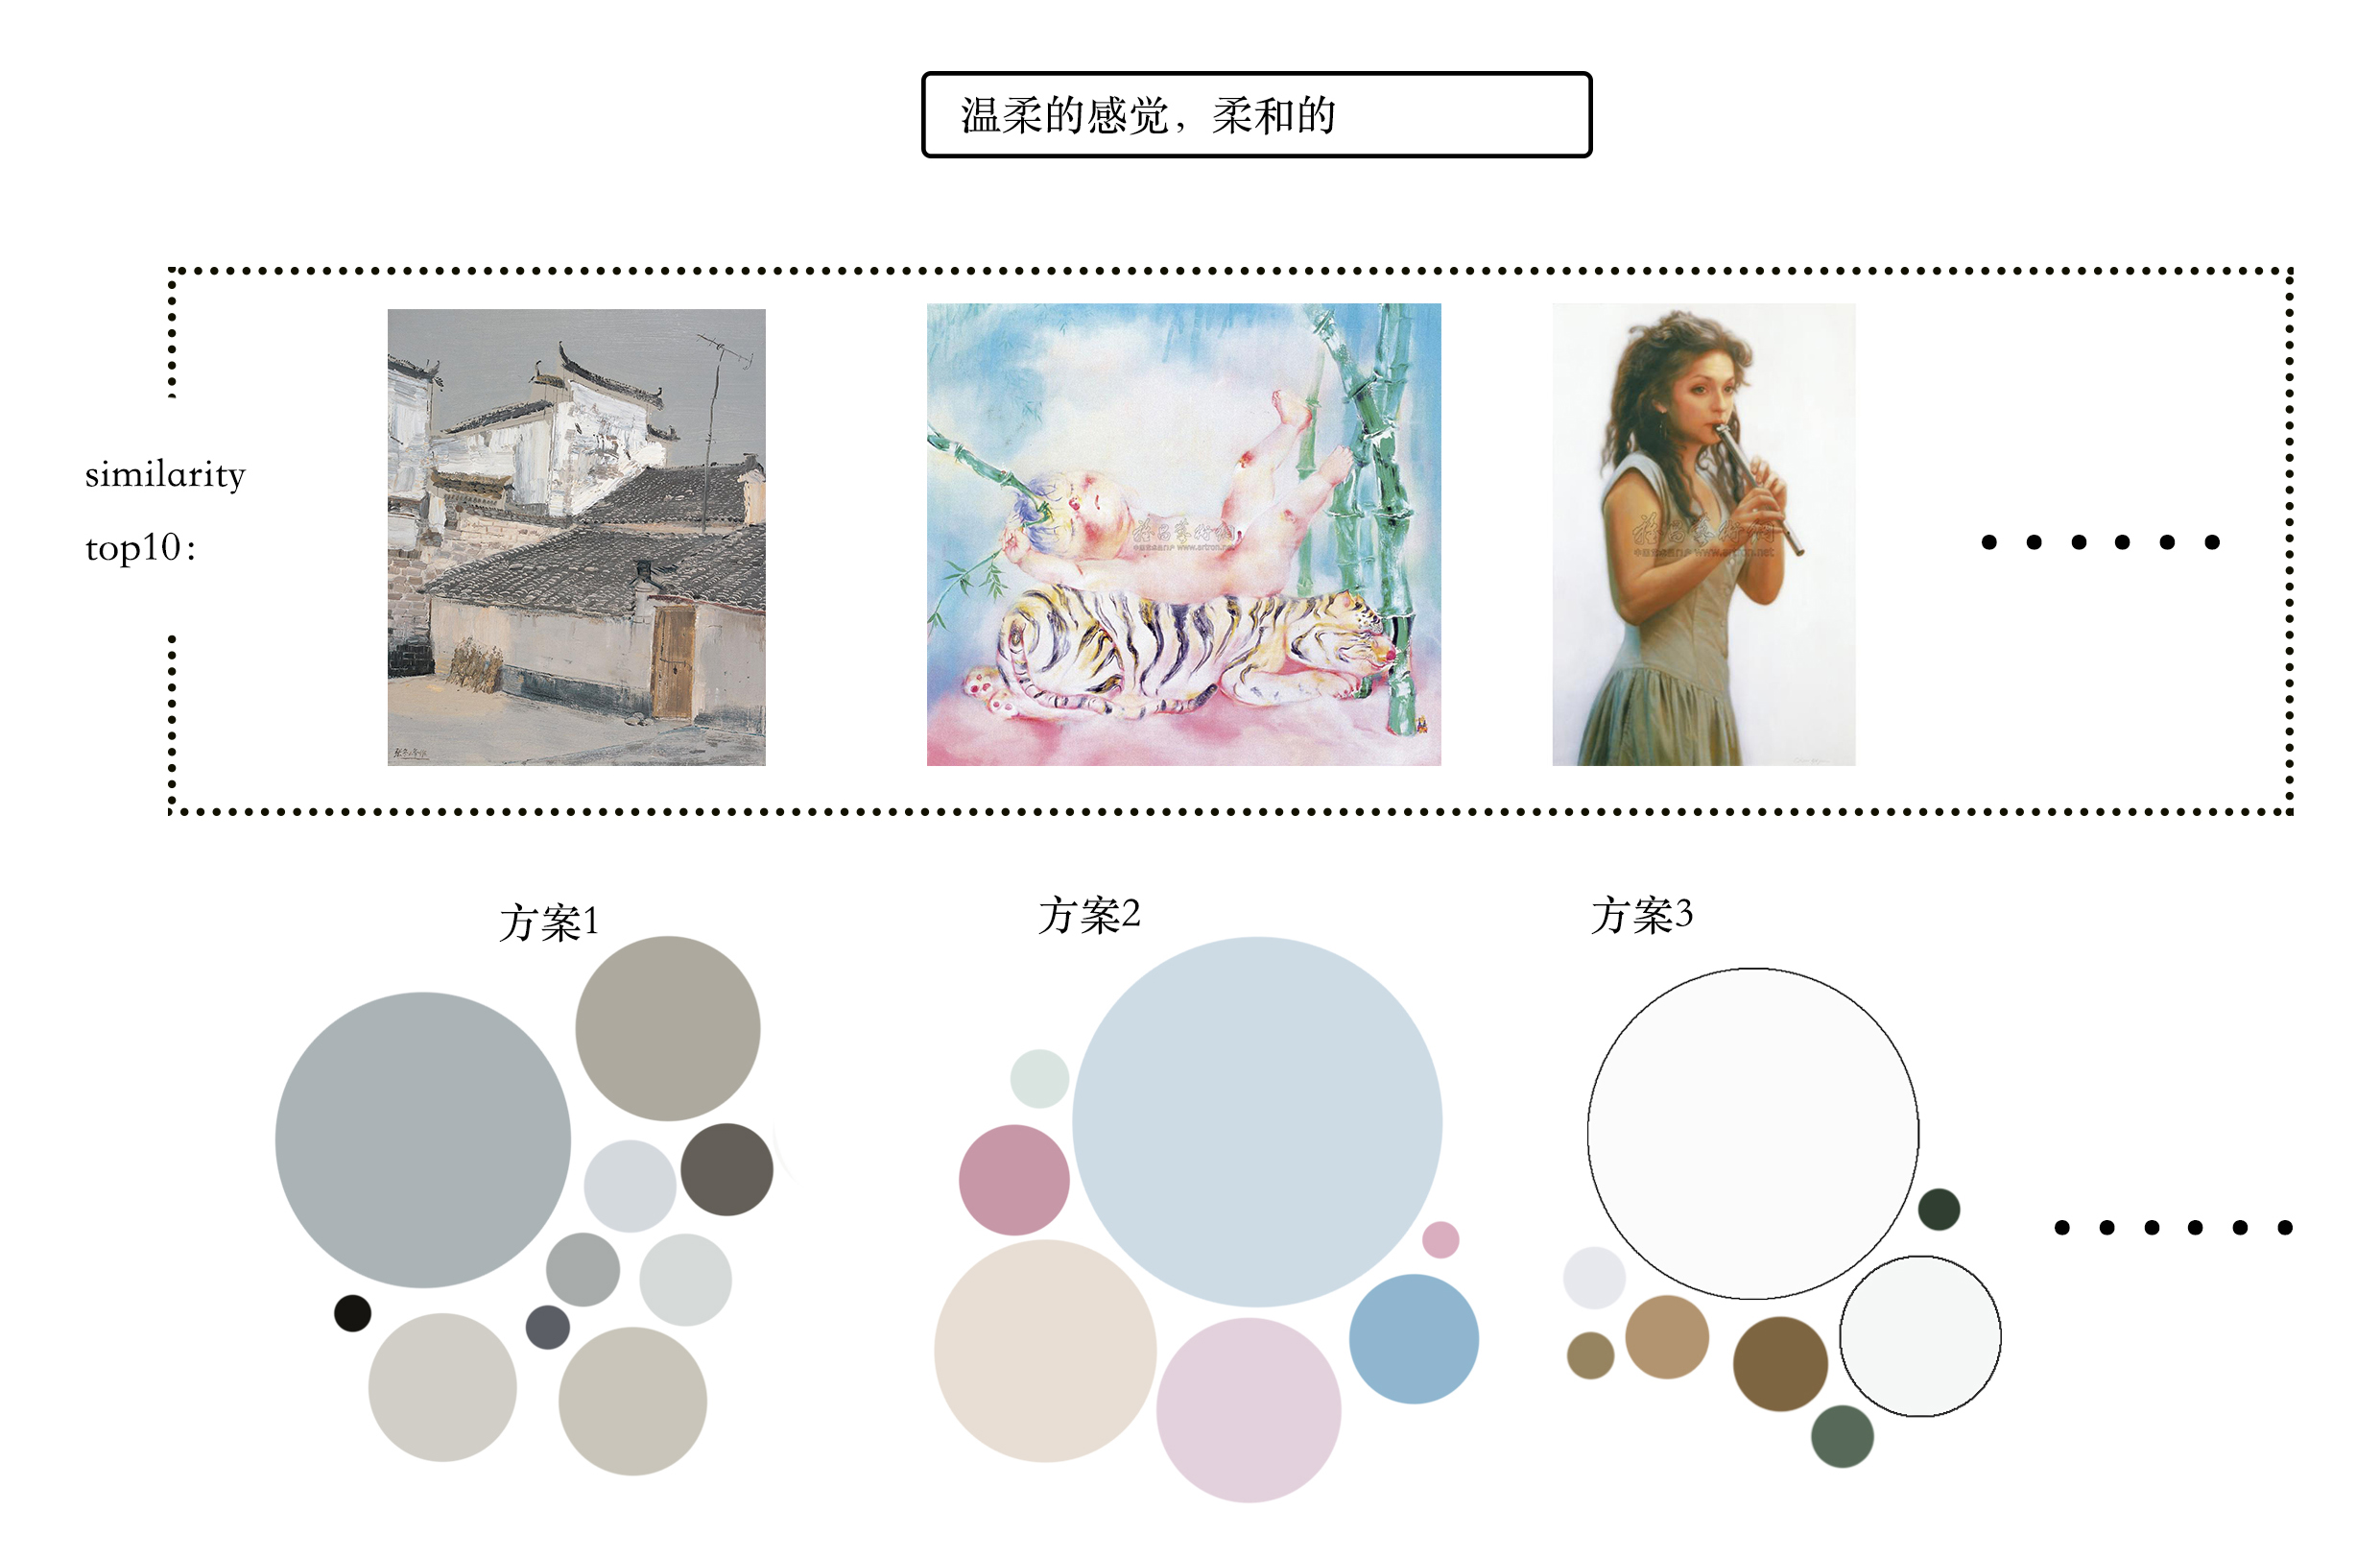
\includegraphics[width=\linewidth,keepaspectratio]{data/chapter-1/搜索结果.jpg}
\caption{备选方案}
\label{figure:搜索结果}
\end{figure}

\subsection{色彩模式}

颜色是不同波长的可见光进入人类的眼睛,由视锥细胞感受到不同波长的比例传到大脑所产生的感受。可见光的波长变化3-5nm,人类就可以分辨为不同的颜色,要对色彩进行数字编码,可以使用多种方法。\cite{colormodel}

RGB色彩模式指Red-Green-Blue三种色光的混合。人类有三种视锥细胞,分别对红、绿、蓝三种色光最为敏感,所以人类的眼睛可以看到的色彩都是由这三种颜色的光经不同比例构成的。光的混合在牛顿时代就被发现了,使用红、绿、蓝三种色适当混合,可以引起光谱上所有任何颜色的感觉,三原色混合原理广泛地应用于照相、显示技术中。数字化常见的颜色标准也使用红、绿、蓝三个通道混合,称为RGB色彩模式。通常情况下,RGB各有256级亮度,用数字表示为从0、1、2...直到255。比如(255,0,0)指红色,(255,255,0)则是黄色,(0,0,0)是三种色光的亮度都为0,即黑色,(255,255,255)是三种色光的亮度都为最高,混合起来为白色。在计算机领域RGB色彩模式是很常用的,需要注意的是,在编码时有时会使用BGR模式,意思并没有区别,但是数字的顺序是反过来的,RGB(255,0,0)为红色而BGR(255,0,0)为蓝色。

常用的色彩模式还有CMYK,多用于印刷,CMYK同样将颜色分为数个通道混合,但是通道为Cyan(青色)-Magenta(品红)-Yellow(黄色)-black(黑色)四个,这四种颜色的染料可以调配出几乎所有颜色。CMYK和RGB色彩模式可以相互转化,转化的方式如下。

\begin{python}
def rgb_to_cmyk(r,g,b):
	cmyk_scale = 100
    if (r == 0) and (g == 0) and (b == 0):
        # black
        return 0, 0, 0, cmyk_scale
    # rgb [0,255] -> cmy [0,1]
    c = 1 - r / 255.
    m = 1 - g / 255.
    y = 1 - b / 255.

    # extract out k [0,1]
    min_cmy = min(c, m, y)
    c = (c - min_cmy) / (1 - min_cmy)
    m = (m - min_cmy) / (1 - min_cmy)
    y = (y - min_cmy) / (1 - min_cmy)
    k = min_cmy

    # rescale to the range [0,cmyk_scale]
    return c*cmyk_scale, m*cmyk_scale, y*cmyk_scale, k*cmyk_scale
\end{python}

关于图像等OpenCV、PIL等库都能够进行转化。在本系统中,所有的色彩都按照RGB模式编码,不同的色彩模式需要进行转化。

\subsection{色彩提取}

色彩提取从图片中占比例最大的颜色开始,可以自定义提取颜色的个数$N_color$,输出的每个颜色包括Red-Green-Blue三个通道的值和该颜色本来在艺术品中占的比例(面积比例)。

色彩提取的算法采用色彩梯度算法。使用RGB色彩模式。首先为了减小计算量通过压缩图像生成一个略缩图。将R-G-B各分为步长为step的n个等级,即总共有$n^3$个颜色等级。对每个颜色等级的像素点个数进行计数,定义色彩c的分数为$score(c) = (saturation(c) + 0.1) \times count(c) $,其中$saturation(c)$为色彩的饱和度,$count(c)$则为颜色为x的像素点个数。非常接近白色的颜色(RGB三个参数均大于200的颜色)和非常接近黑色的颜色(三个参数均小于50的颜色)都不参加评分。面积越大、色彩饱和度越高,则色彩得分越高。得分越高的颜色就是图片中主要的颜色,提取前$N_color$个得分最高的颜色,$count(c)$就代表这这个颜色在艺术品中占的比例。

\begin{python}
def get_dominant_color(image, beside_color, step):  
      
#颜色模式转换,以便输出rgb颜色值  
    image = image.convert('RGBA')  
      
#生成缩略图,减少计算量 
    image.thumbnail((200, 200))  
      
    max_score = 0 
    dominant_color = 0  
    proportion = 0
        
    for count, (r, g, b, a) in image.getcolors(image.size[0] * image.size[1]):  
        # 跳过透明色  
        if a == 0:  
            continue
        # 跳过白色    
        if ((r>180)&(g>180)&(b>180)):  
            continue
        # 跳过黑色   
        if ((r<80)&(g<80)&(b<80)):  
            continue 
            
        if ((beside_color[0]-step<r<beside_color[0]+step)&(beside_color[1]-step<g<beside_color[1]+step)&(beside_color[2]-step<b<beside_color[2]+step)):  
            continue
               
        saturation = colorsys.rgb_to_hsv(r / 255.0, g / 255.0, b / 255.0)[1]          
        y = min(abs(r * 2104 + g * 4130 + b * 802 + 4096 + 131072) >> 13, 235)         
        y = (y - 16.0) / (235 - 16)  
          
        # 忽略高亮色  
        if y > 0.9:  
            continue  

        score = (saturation + 0.1) * count  
          
        if score > max_score:  
            max_score = score  
            dominant_color = (r, g, b)  
            proportion = count
      
    return dominant_color, proportion  
\end{python}

这样的方式略过黑色和白色(或者说几乎是黑色和白色的颜色),面积越大、色彩饱和度越高,色彩越排在前面,可以完全忠实于艺术品图片提取色彩。

\section{上色算法}

\subsection{系统结构之自动上色}

从艺术品中提取色彩之后,色彩方案可以自动在效果图线稿上预览。上色预览主要是为了让设计师直观的到色彩方案的风格和潜力,为了满足这个目标有3点需求:1.快速实时;2.色彩准确和比例较准确;3.效果图清晰明确。

\begin{figure}[!htbp]
\centering
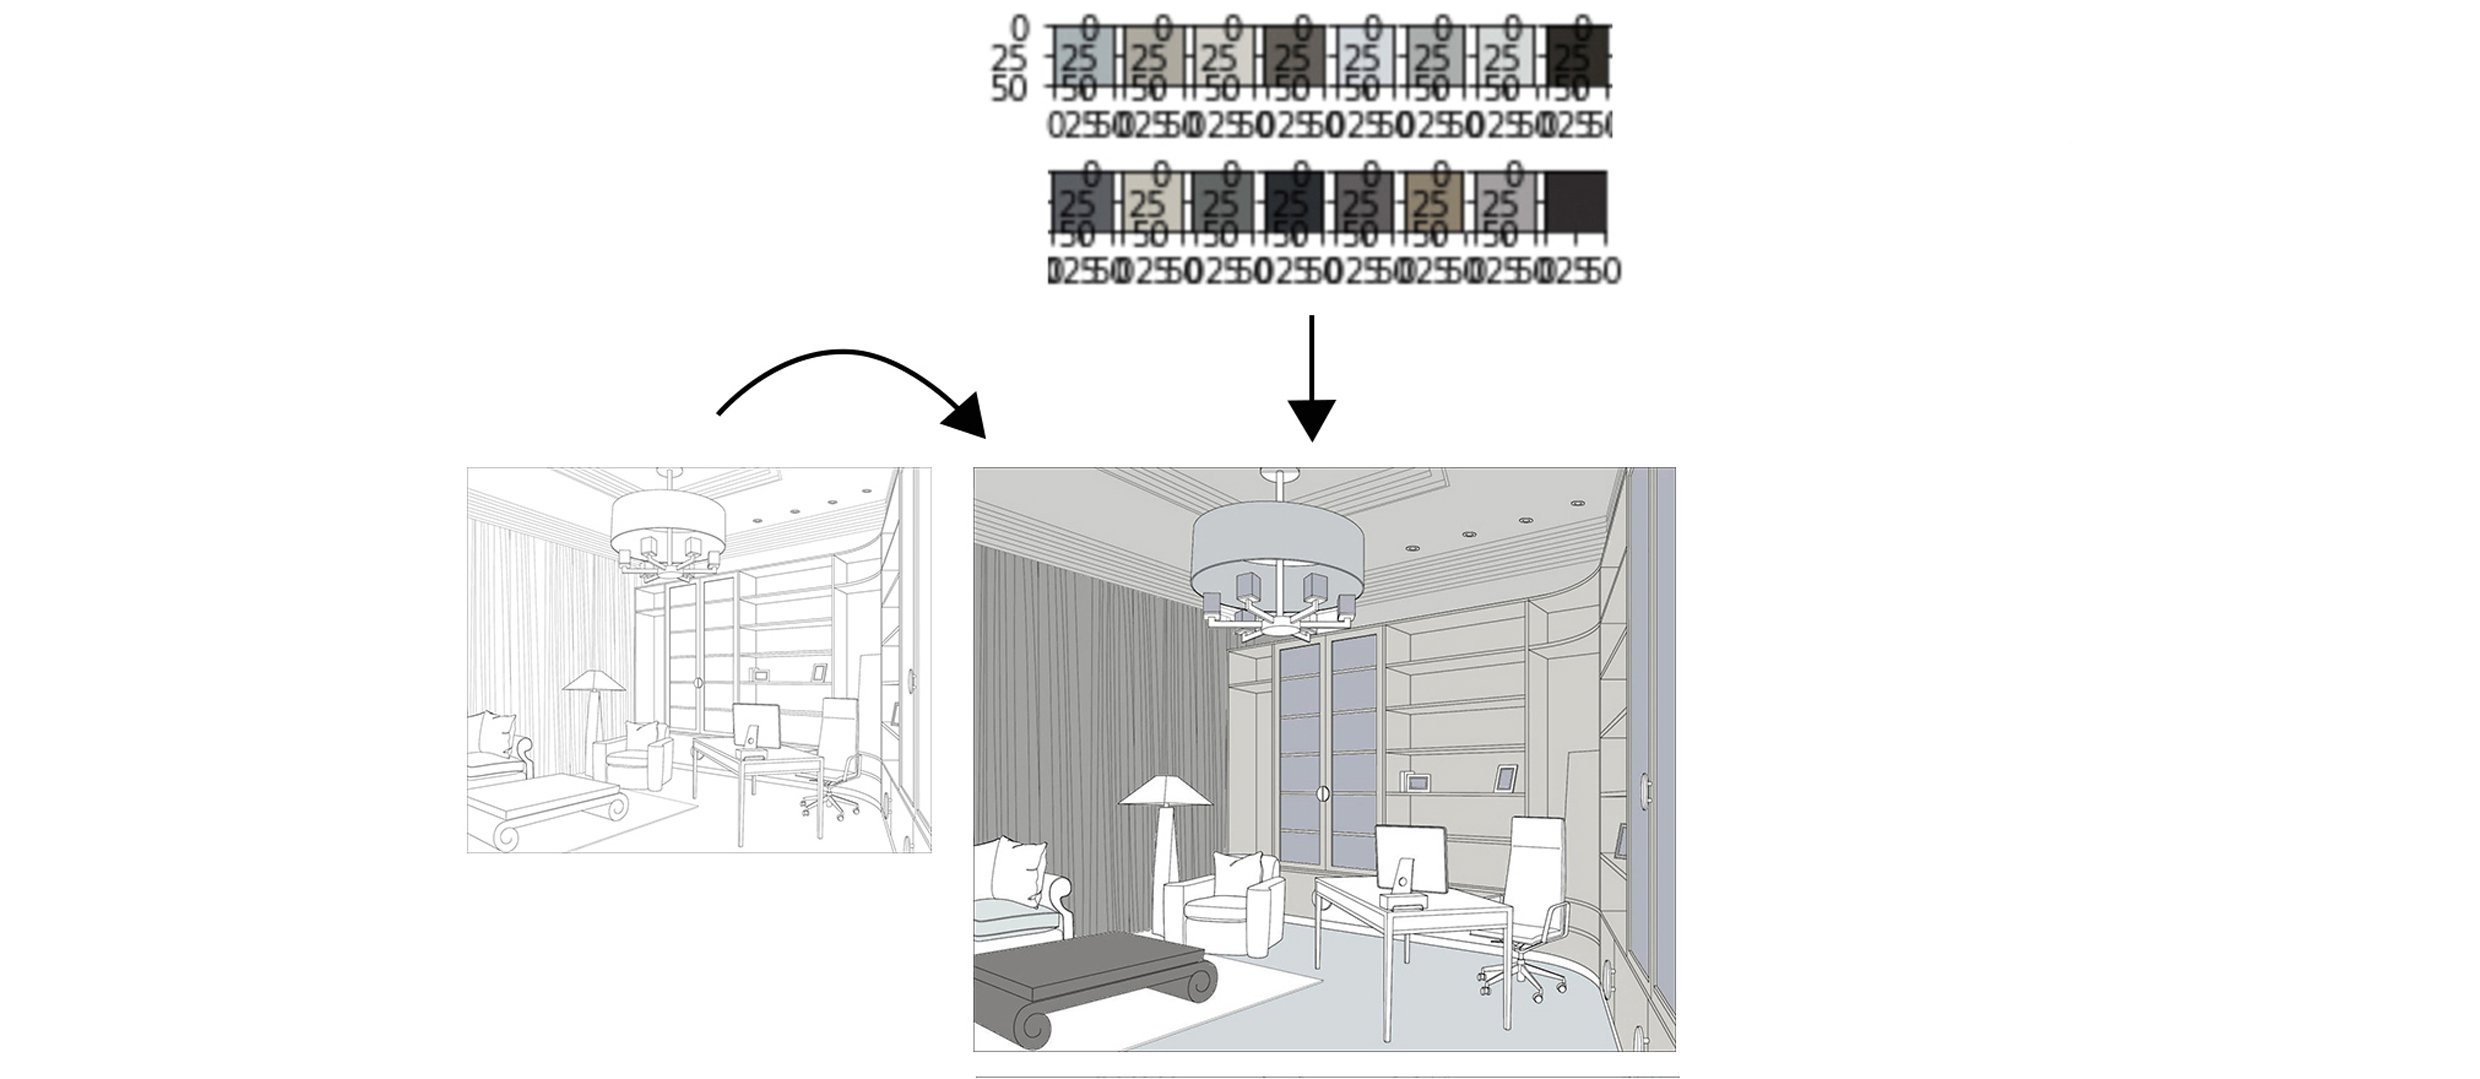
\includegraphics[width=\linewidth,keepaspectratio]{data/chapter-1/系统内部逻辑3.jpg}
\caption{第三步:自动上色}
\label{figure:系统内部逻辑提取}
\end{figure}

系统准备了室内设计,服装设计各1套效果图线稿预览,之后的测试发现,对于上色区域占图片比例较小并且色彩有限的服装、产品效果图本系统也可以使用,但系统效果更适合室内设计效果图。每次生成的预览效果图由于有随机性的参与都不可复制,但可以使用同一色彩方案生成不完全一致但风格同一的预览图。

\subsection{泛洪填充算法}

泛洪填充算法(Flood Fill Algorithm)又称漫水填充算法,是在很多图形绘制软件中常用的填充算法。\cite{floodfill} 泛洪填充算法可以为图像的封闭区域填充颜色,成完整的填充需要的条件有两点:1.该区域有封闭的边界;2.该区域的像素点色彩相同。如图~\ref{figure:泛洪填充}。

\begin{figure}[!htbp]
\centering
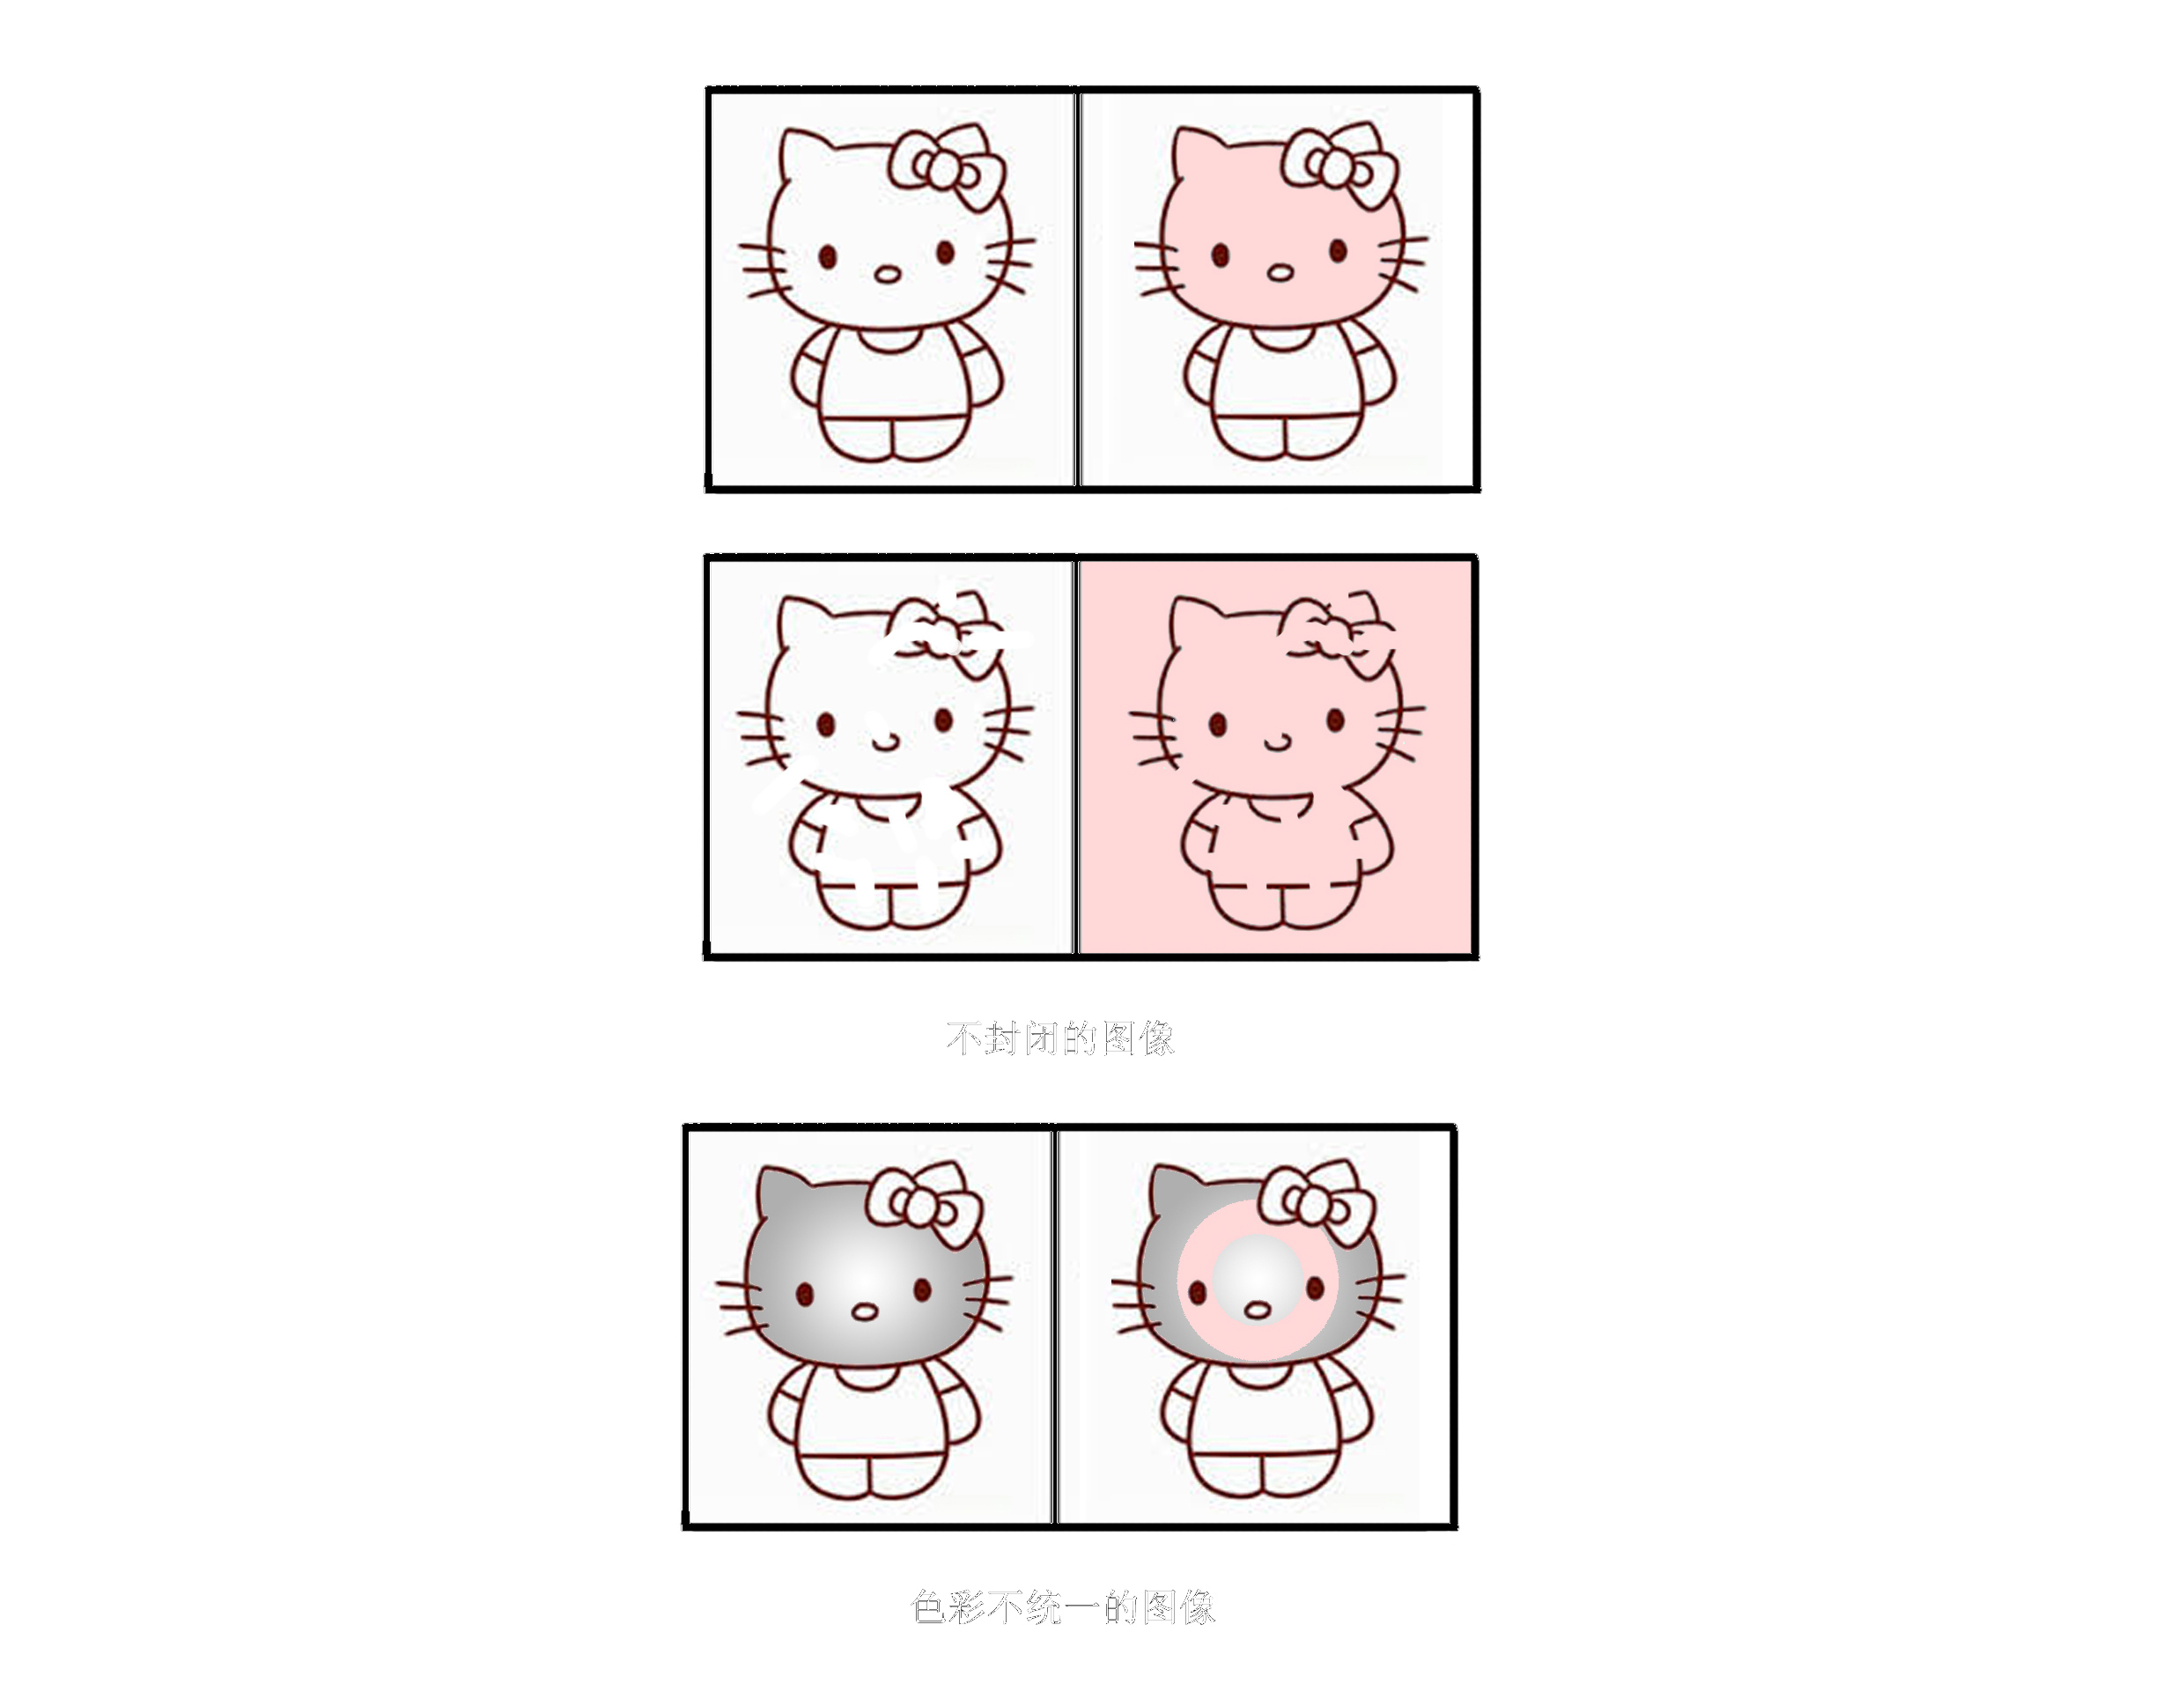
\includegraphics[width=\linewidth,keepaspectratio]{data/chapter-1/kitty.jpg}
\caption{泛洪填充}
\label{figure:泛洪填充}
\end{figure}

泛洪填充算法的原理是,要为某个区域填充色彩a,在这个区域中取一个像素点,这个点被称为种子点,种子点原始的颜色为x,将种子点的色彩从x改为a,对于所有相邻且颜色为x的点也都染色为a,染色后的点相邻且颜色为x的点也都染色为a,一直传播下去,直到这个区域内所有的点都被填充完为止。如图~\ref{figure:填充过程}。

\begin{figure}[!htbp]
\centering
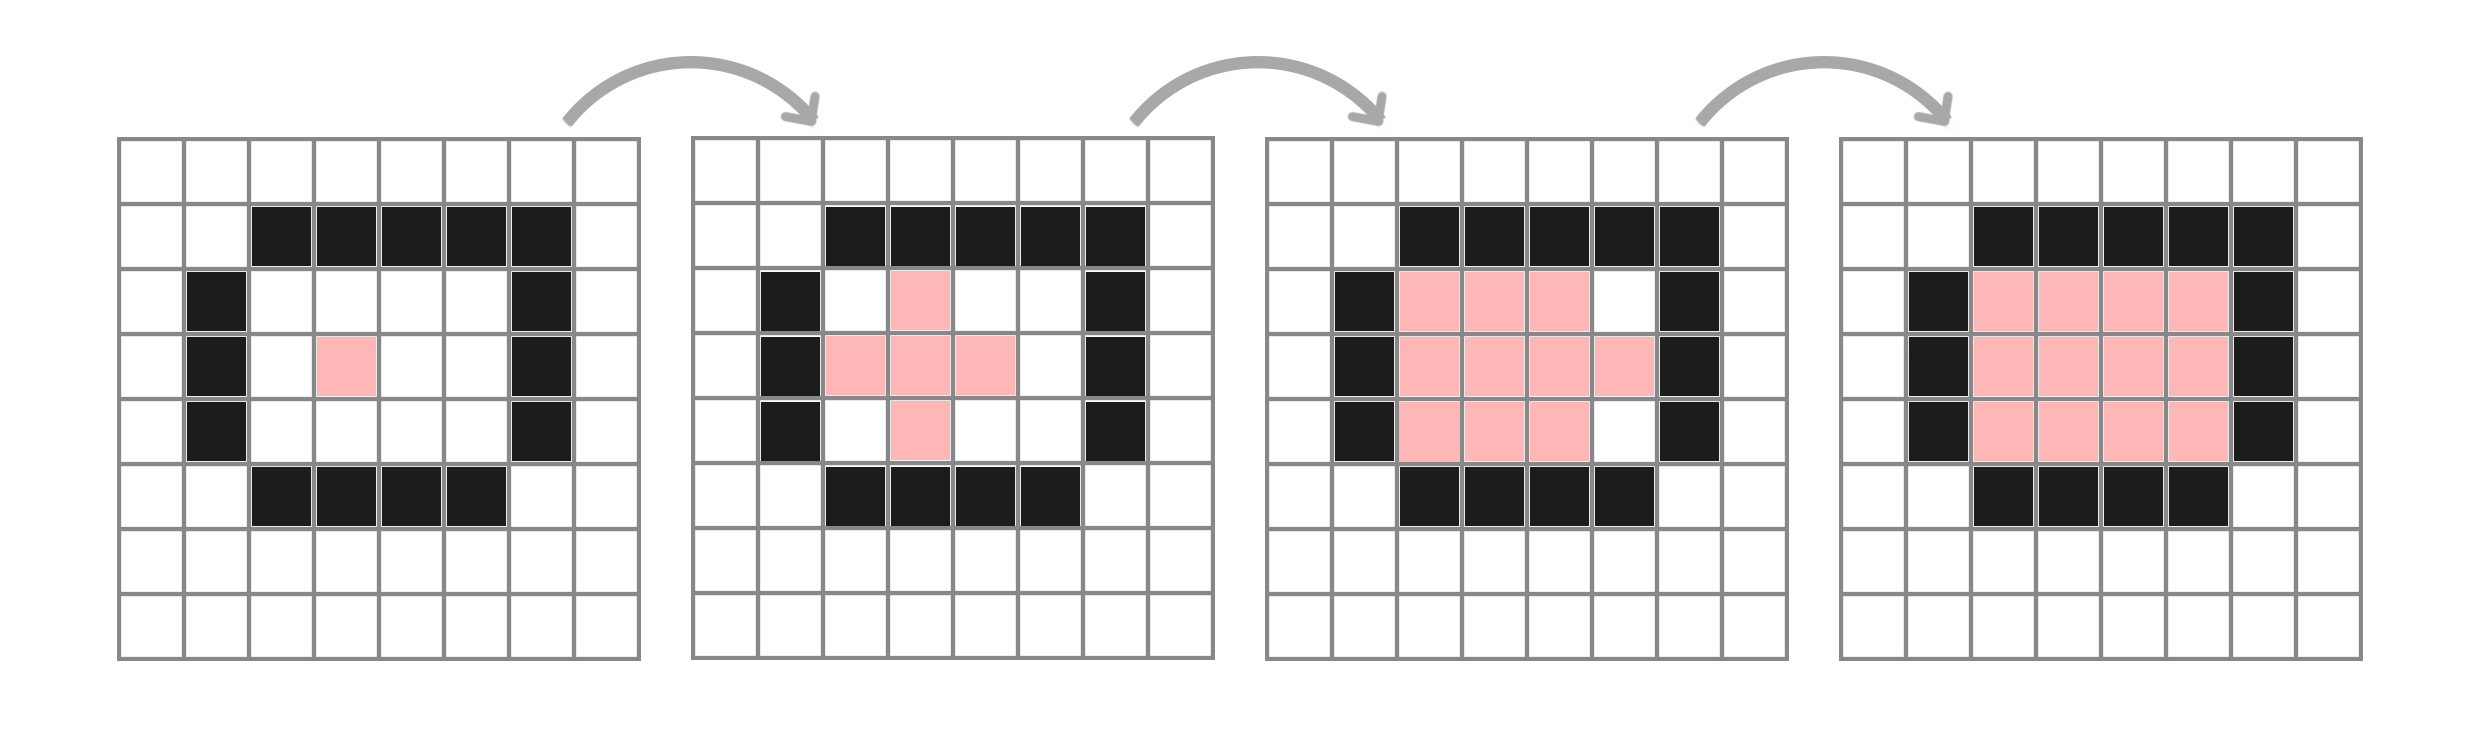
\includegraphics[width=\linewidth,keepaspectratio]{data/chapter-1/填充.jpg}
\caption{填充过程}
\label{figure:填充过程}
\end{figure}

实现这样的算法只需要最基础的递归算法或堆栈算法。即
\begin{python}
def floodfill(x, y, oldColor, newColor):
    # assume surface is a 2D image and surface[x][y] is the color at x, y.    
    if surface[x][y] != oldColor: return # the base case
    surface[x][y] = newColor
    floodfill(x + 1, y, oldColor, newColor) # right
    floodfill(x - 1, y, oldColor, newColor) # left
    floodfill(x, y + 1, oldColor, newColor) # down
    floodfill(x, y - 1, oldColor, newColor) # up
\end{python}

在实际的使用中,这个简单的算法还需要一些改进。复制制作一个遮罩层,以防图片被直接改变导致返回结果不正常。加入容差的概念,即当染色点原始的颜色为最大负差值不超过RGB(20,20,20),最大正差值不超过RGB(50,50,50),则可以扩散。

在本系统中,待上色的效果图为室内设计效果图,通过随机选点来为设计效果图上色。每次上色的程序如下:随机选取效果图中像素点,如果这个点为白色则填充当前色彩,同时替换当前色彩为色彩列表下一个色彩;如果这个点非白色,则再次随机选取效果图中的像素点。使用的色彩列表为从艺术品提取的色彩方案,色彩按艺术品中色彩的比例从高到低排序,循环排列,循环多次,直到图片上色完整。

\subsection{一些问题}

\subparagraph{漏掉到小面积——随机游走}:
使用泛洪填充算法可以非常准确工整的为室内设计效果图线稿上色,完全的随机取点会使某些较小的面积被选中的概率太小,所以无法上色的情况严重,如图~\ref{figure:漏掉上色面积的问题以及解决办法}(a)图像中很多地方没有成功上色。

\begin{figure}[!htbp]
\centering
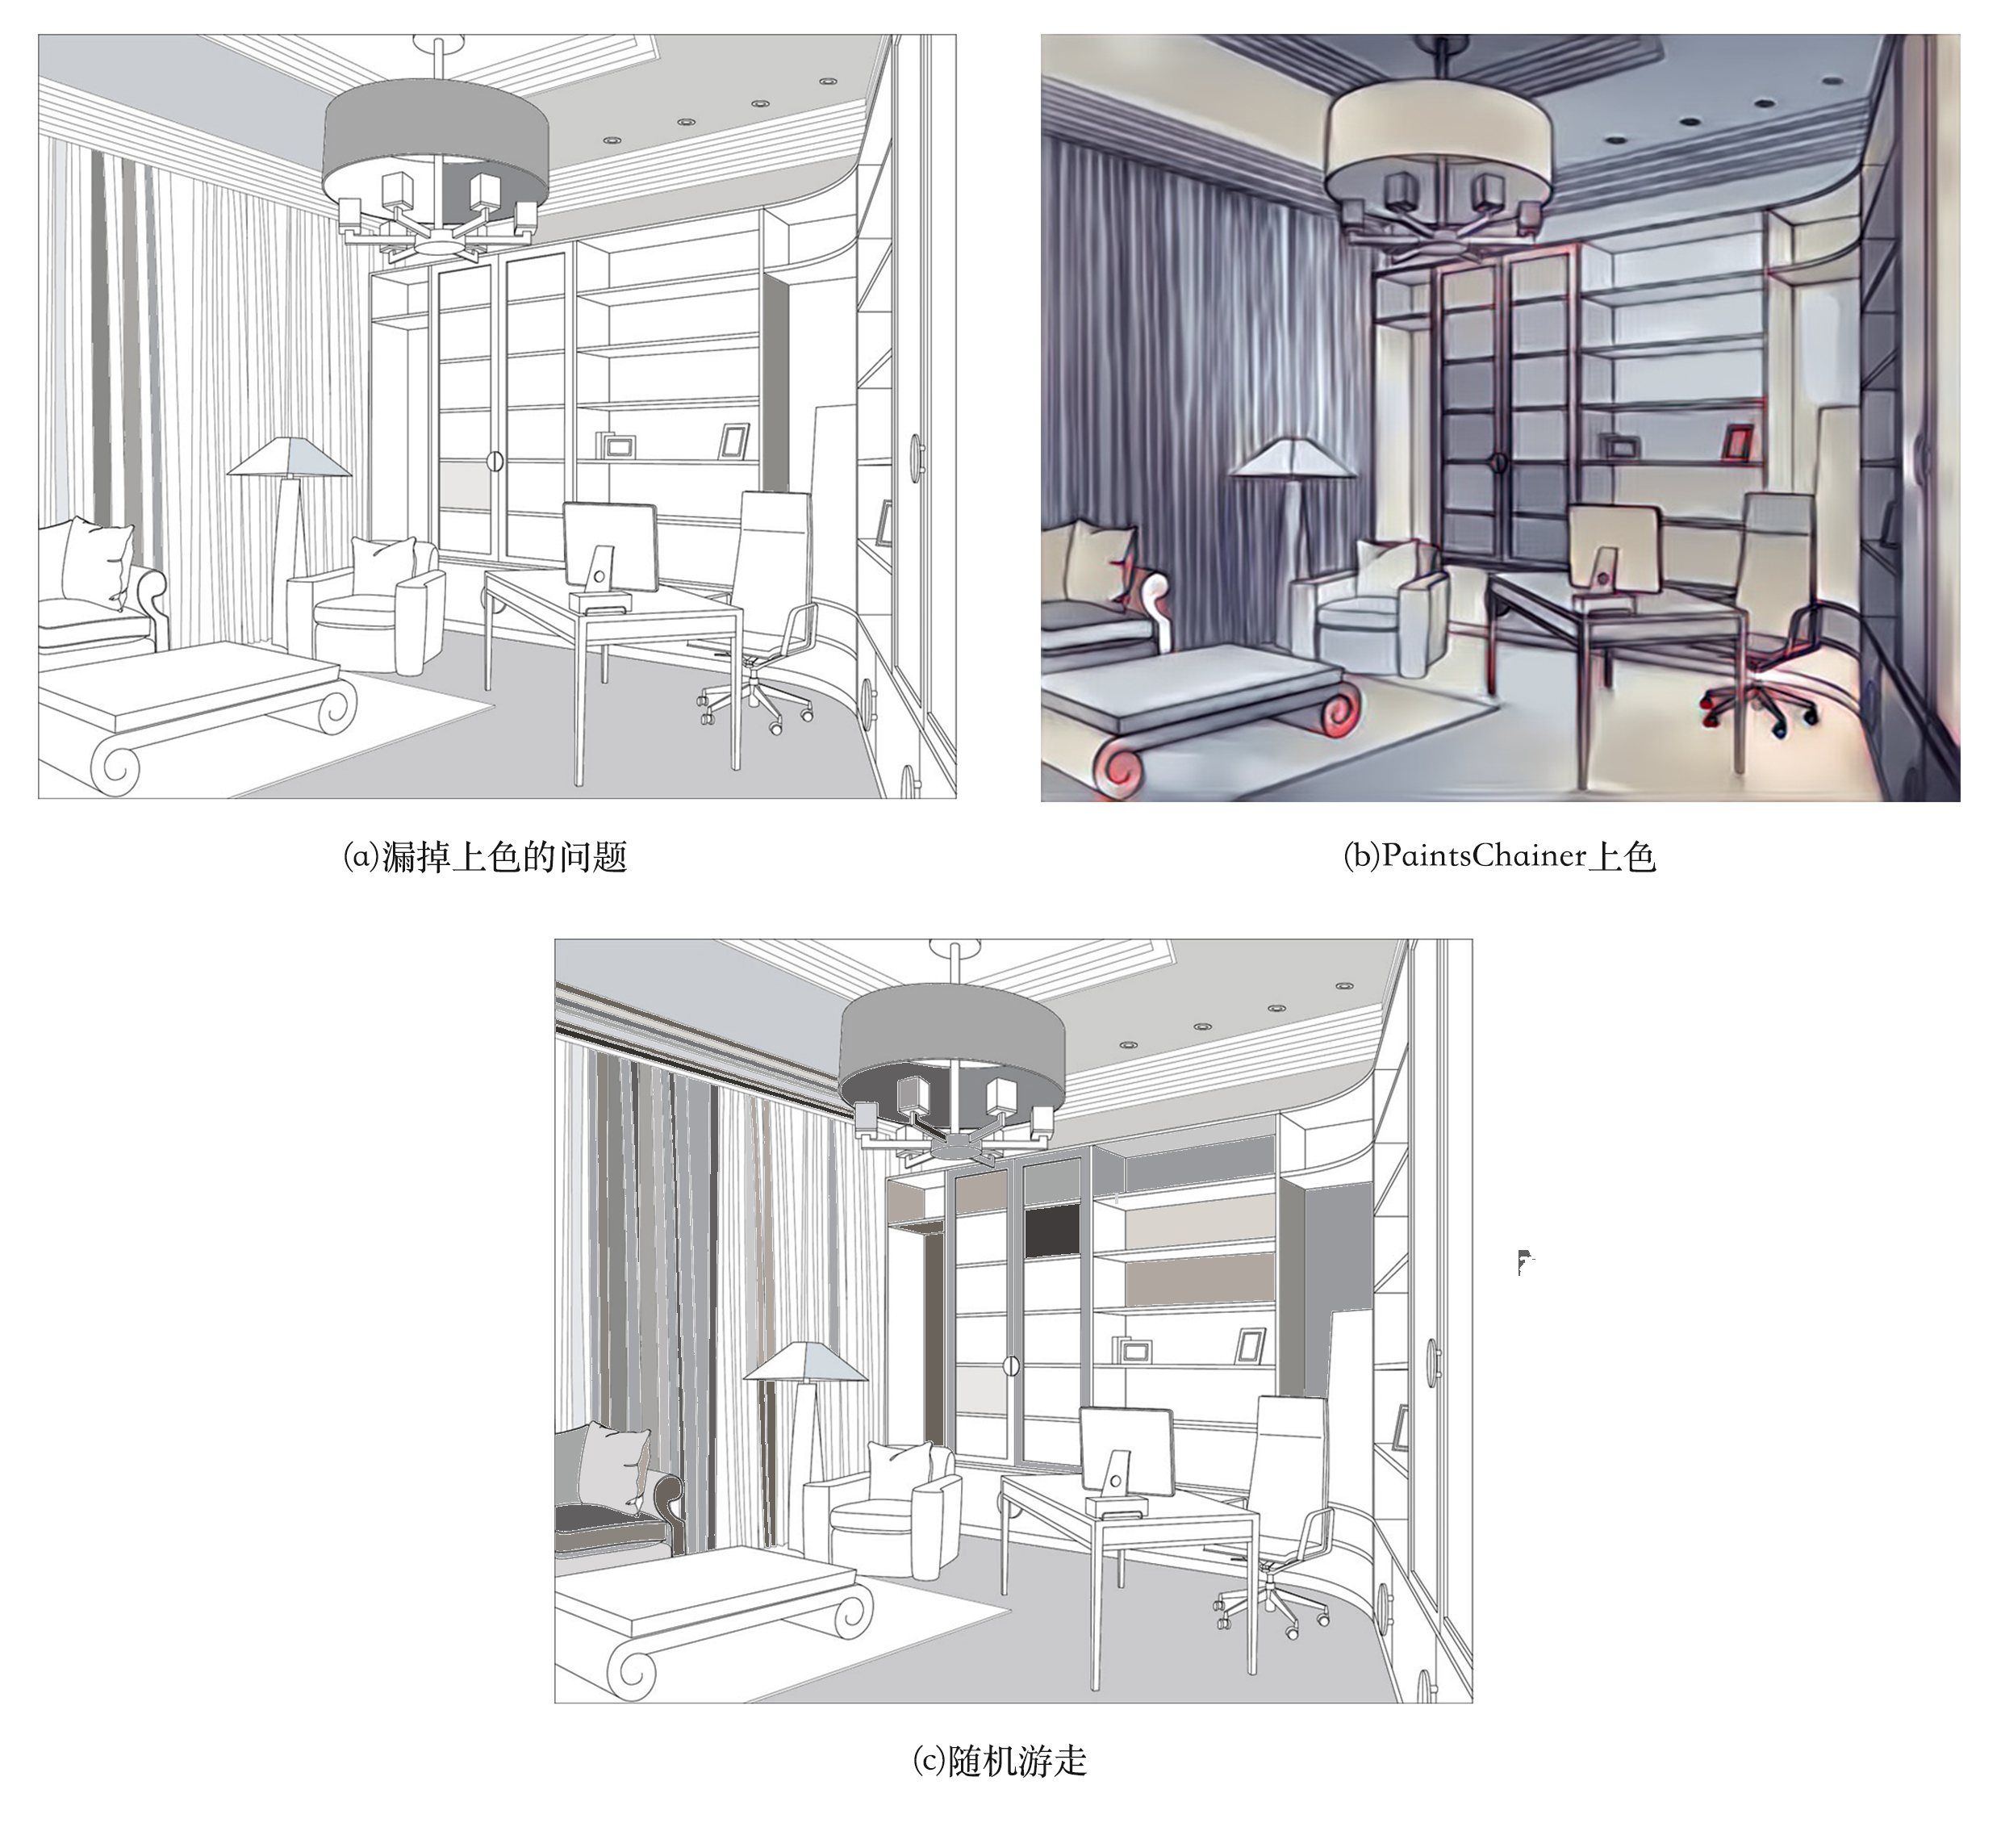
\includegraphics[width=\linewidth,keepaspectratio]{data/chapter-1/预览2.jpg}
\caption{漏掉上色的问题}
\label{figure:漏掉上色面积的问题以及解决办法}
\end{figure}

为了解决这个问题,PaintsChainer所采用的神经网络算法的可以完全的给整张图片上色,如图~\ref{figure:漏掉上色面积的问题以及解决办法}(b)但是对于即时预览色彩方案的效果图来说,不工整的上色、混色、神经网络生成的错误阴影导致预览色彩改变并不适合本系统的需要。生成图像的数十秒延迟也是这个算法不合适的原因。

在原来的方法上面可做一些改进使用随机游走的方式,完全的随机取点会使某些较小的面积被选中的概率太小,无法上色。使用随机游走的方式改进上色算法可以更少出现漏掉面积较小的区域的情况。随机游走的方式倾向于一个区间接一个区间的上色,如图~\ref{figure:漏掉上色面积的问题以及解决办法}(c),循环次数足够多的情况下可以起到更好的效果。

\subparagraph{色彩连续性——图片预处理}:

使用洪填充算法会出现这样的问题,例如区域1和区域2都是天花板,一般而言是同种颜色,但是
现在的填充算法一点也不懂这件事。

\begin{figure}[!htbp]
\centering
\includegraphics[width=\linewidth,keepaspectratio]{data/chapter-1/预2.jpg}
\caption{色彩连续性的问题}
\label{figure:漏掉上色面积的问题}
\end{figure}

所以将这个效果图进行一点预处理,这样可以基本保证在每个完整的物体会填充同一种色彩。预处理的方式是通过标注的方式将同一物体的信息提取出来,删去物体内部的线条,保留物体的的外轮廓。与此同时我们还可以做一些其他的标注,比如将透明的物体的色彩标注为某个灰色。之后再进行填充,就可以将同一个物体填充一个颜色。最后,再通过图层叠加的方式将效果图的原线稿叠加在上色稿上,得到最终的效果图。

\begin{figure}[!htbp]
\centering
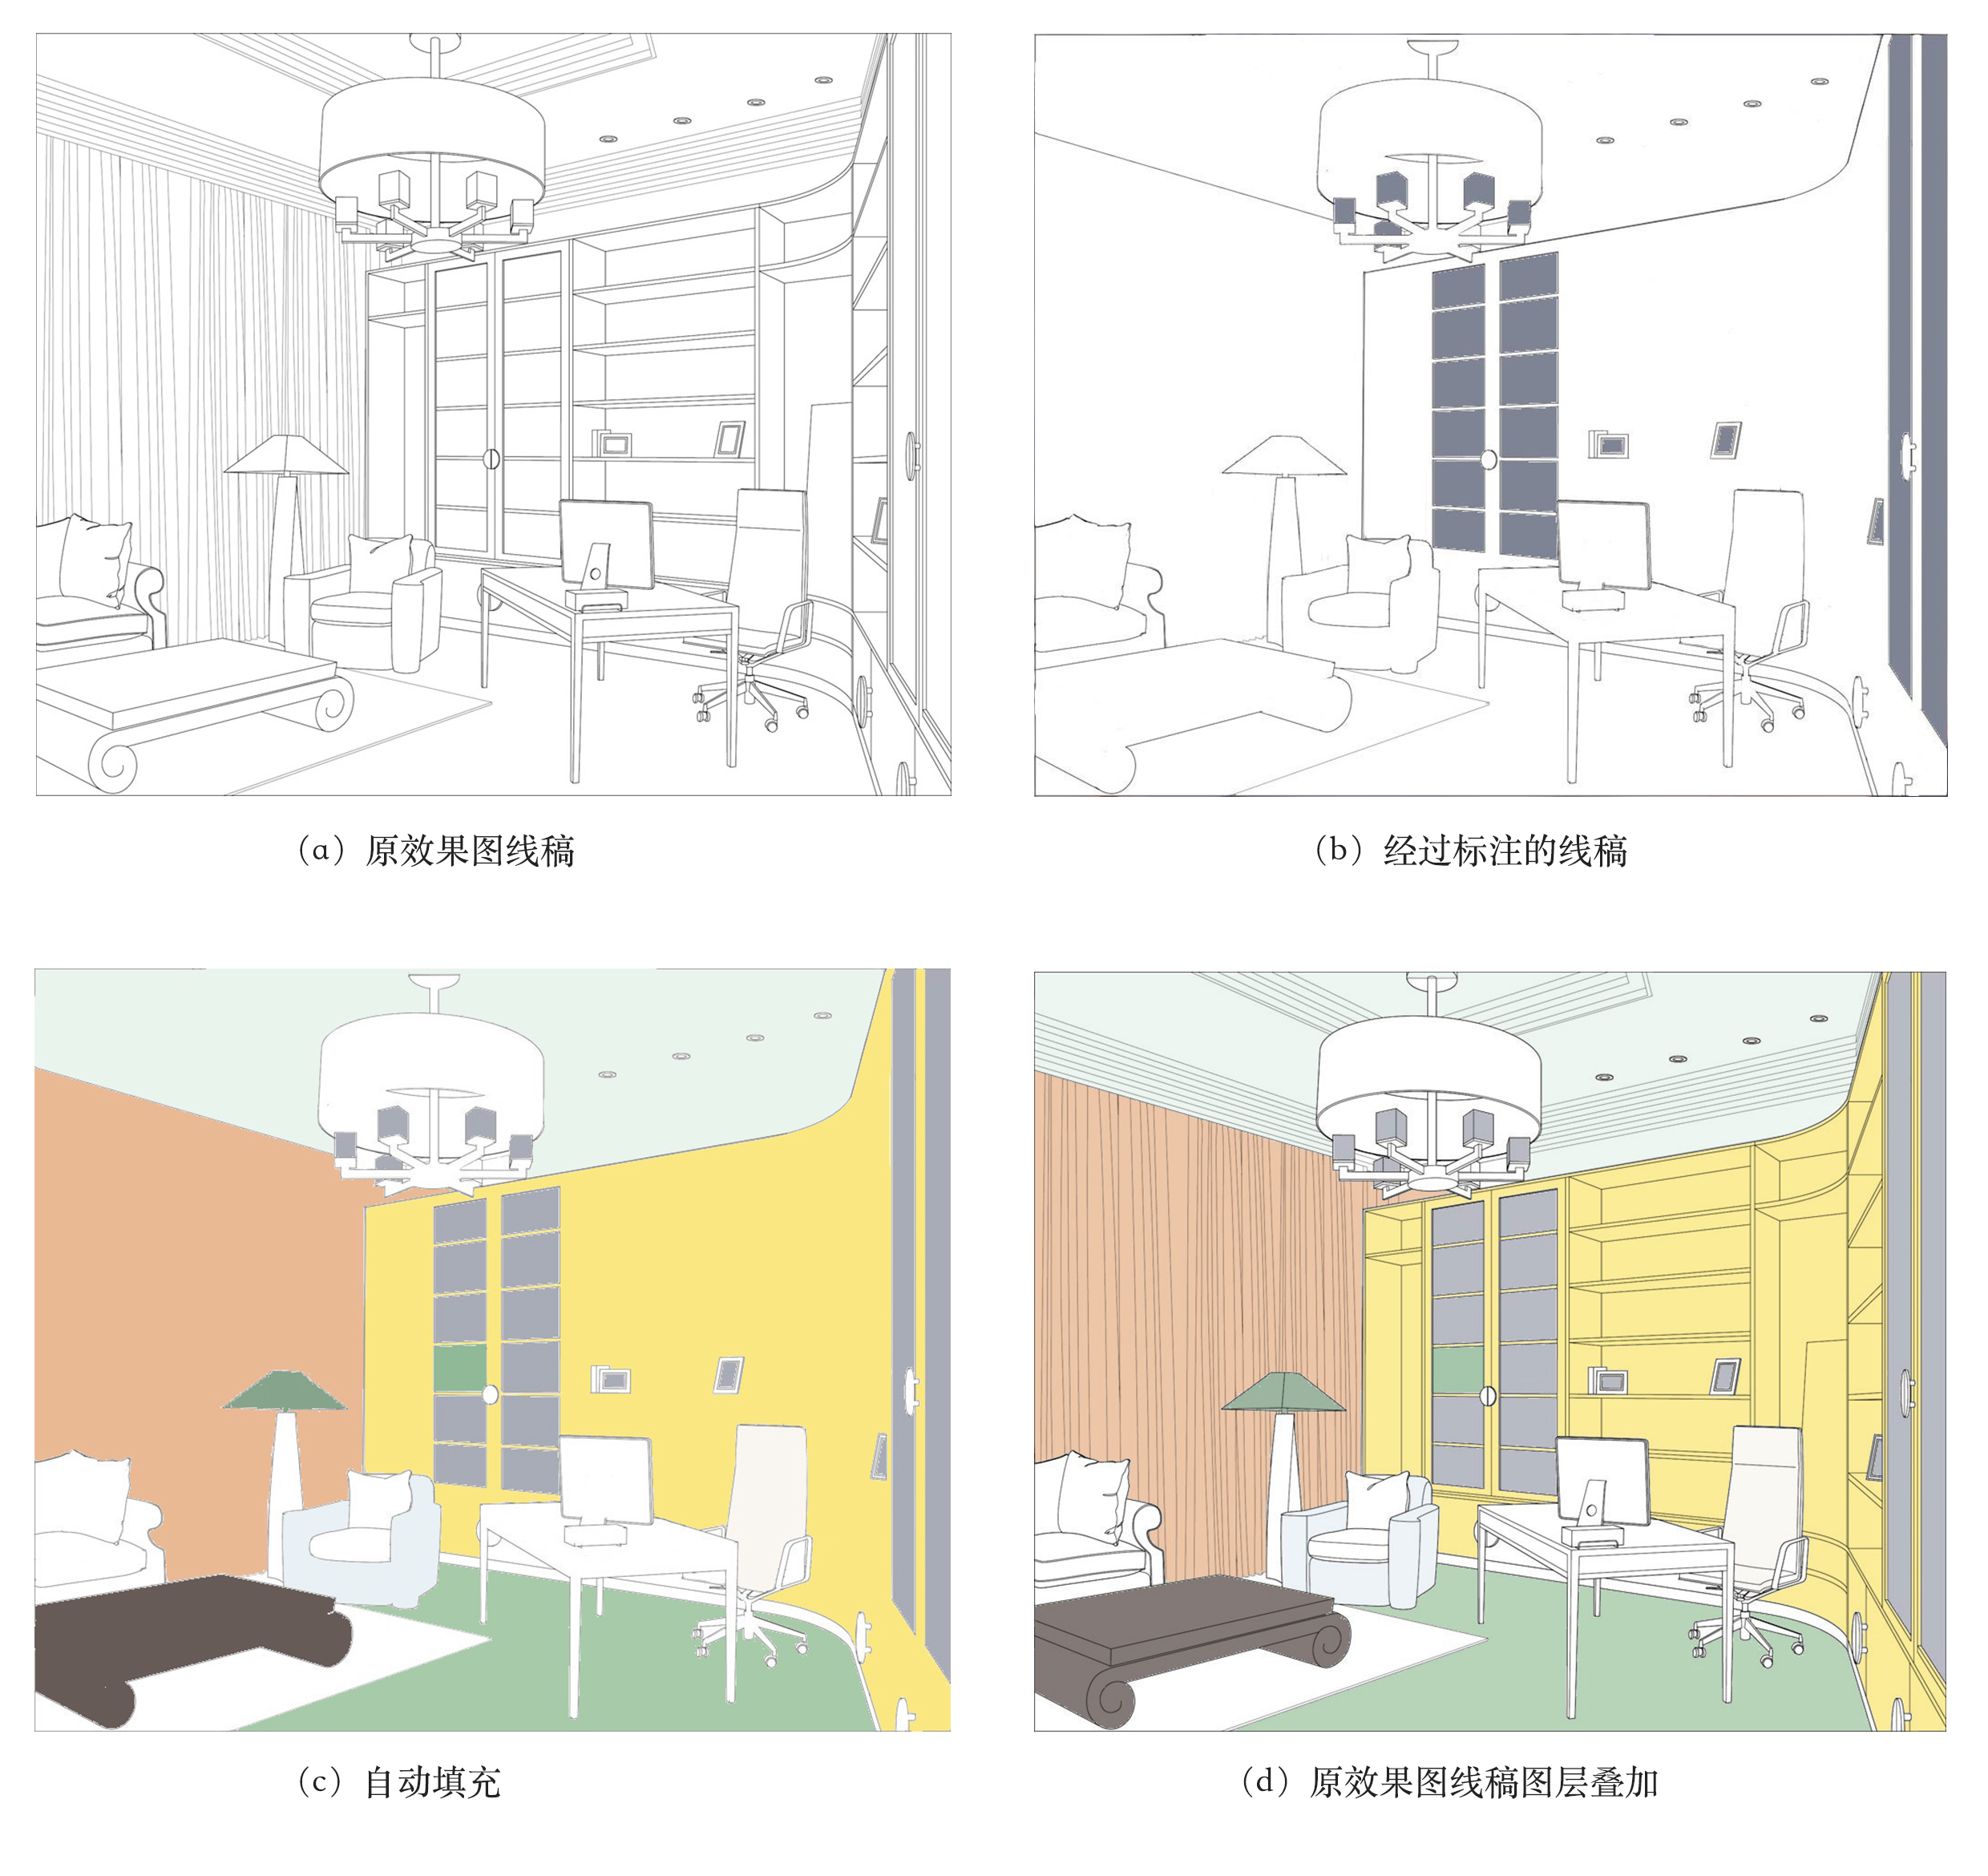
\includegraphics[width=\linewidth,keepaspectratio]{data/chapter-1/预览2副本.jpg}
\caption{色彩连续性的处理}
\label{figure:漏掉上色面积的问题}
\end{figure}


%\subsection{色彩比例}

%对于区域$i$,在效果图上的面积占比为$P_i$,则随机选择种子点在区域$i$的可能性也为$P_i$。对于色彩$j$,在原艺术品上占比例为$p_j$。

\section{本章小结}

本系统的整体思路为:1.输入对需求的文本描述;2.针对输入语句对艺术品的文本信息进行语义搜索,找出与之关联度高的艺术品文本信息;3一句艺术品数据库中艺术品的图片信息和文本信息的隐藏存词关联匹配对应,找出与输入文本关联度高的图片;4.从图片中提取色彩方案,包括绘画作品的色彩和配色比例;5将所提取的色彩运用到设计效果图上预览。

对于用户来说,本系统的使用方式如下:1.用户输入对需求的文本描述;2.得到配色方案;3.当用户不满于当前色彩方案可以重新搜索;4.使用当前色彩方案为效果图上色;5.当用户不满于当前效果图可以使用当前色彩方案重新上色。

在实现的过程中,首先需要解决的是自然语言处理的问题。本系统采用word embedding的方式实现单词向量化,word embedding采用CBOW模型,使用哈夫曼树、负采样优化、fast text等策略加快速度以及增加编码的精度,实现对词语语义信息的提取。词向量到句向量的转化采用加权合成的方法,考虑词频、类型权重等实现对句子的精准建模,将句子中重要的语义信息提取出来,略去系统不关心的信息,建立艺术品文本信息句向量词典。使用余弦相似度作为指标,在词典中寻找与输入句子匹配的艺术品。之后需要对图像进行处理,从匹配的艺术品图片中提取色彩。最后对效果图自动上色。

整个系统运行的过程相应迅速,匹配准确,效果图预览清晰有效,可以直接高效的为设计师提供快速的参考和辅助。



